\section{Validaci\'on}

El modelo isot\'ermico de Li ha sido utilizado exitosamente en la simulaci\'on de problemas multif\'asicos diversos, como el impacto de droplets sobre una superficie plana o en la medici\'on de frecuencia de escilaci\'on de droplets aislados. 

\subsection{Construcci\'on de Maxwell}

La inconsistencia termodin\'amica intr\'inseca de los modelos \pp{} obliga a llevar a cabo, como primer paso de verificaci\'on, experimentos num\'ericos destinados a cuantificar la desviaci\'on entre las densidades de coexistencia reproducidas por el modelo y aquellas definidas mediante la regla de construcci\'on de Maxwell. Estos expermentos, conocidos simplemente como de construcci\'on de Maxwell, consisten b\'asicamente en la simulaci\'on de un sistema adecuado, simple, pero que a la vez involucre la fenomenolog\'ia buscada.

En este caso, el problema elegido consiste en la simulaci\'on de una regi\'on bidimensional de $200 \times 200$ unidades de grilla (u.g.), con condiciones de contorno peri\'odicas, temperatura uniforme, sin fuerzas externas, y que inicialmente contiene un fluido con densidad perturbada aleatoriamente en  $\pm 1\%$ alrededor del valor cr\'itico ($\rho=\rho_c$). Como se ejemplifica en la \fig{fig:maxwell_2d}, en los primeros instantes comienzan a generarse regiones de diferente densidad, que contin\'uan separ\'andose y agrup\'andose hasta formar estructuras estacionarias, con densidades claramente diferentes. De esta manera, pueden tomarse los valores de densidad en el interior de cada fase, lejos de las interfases, y compararlos con los determinados por la regla de Maxwell.

\begin{figure}[htb]
    \centering
    \begin{subfigure}[t]{0.45\textwidth}
        \centering
        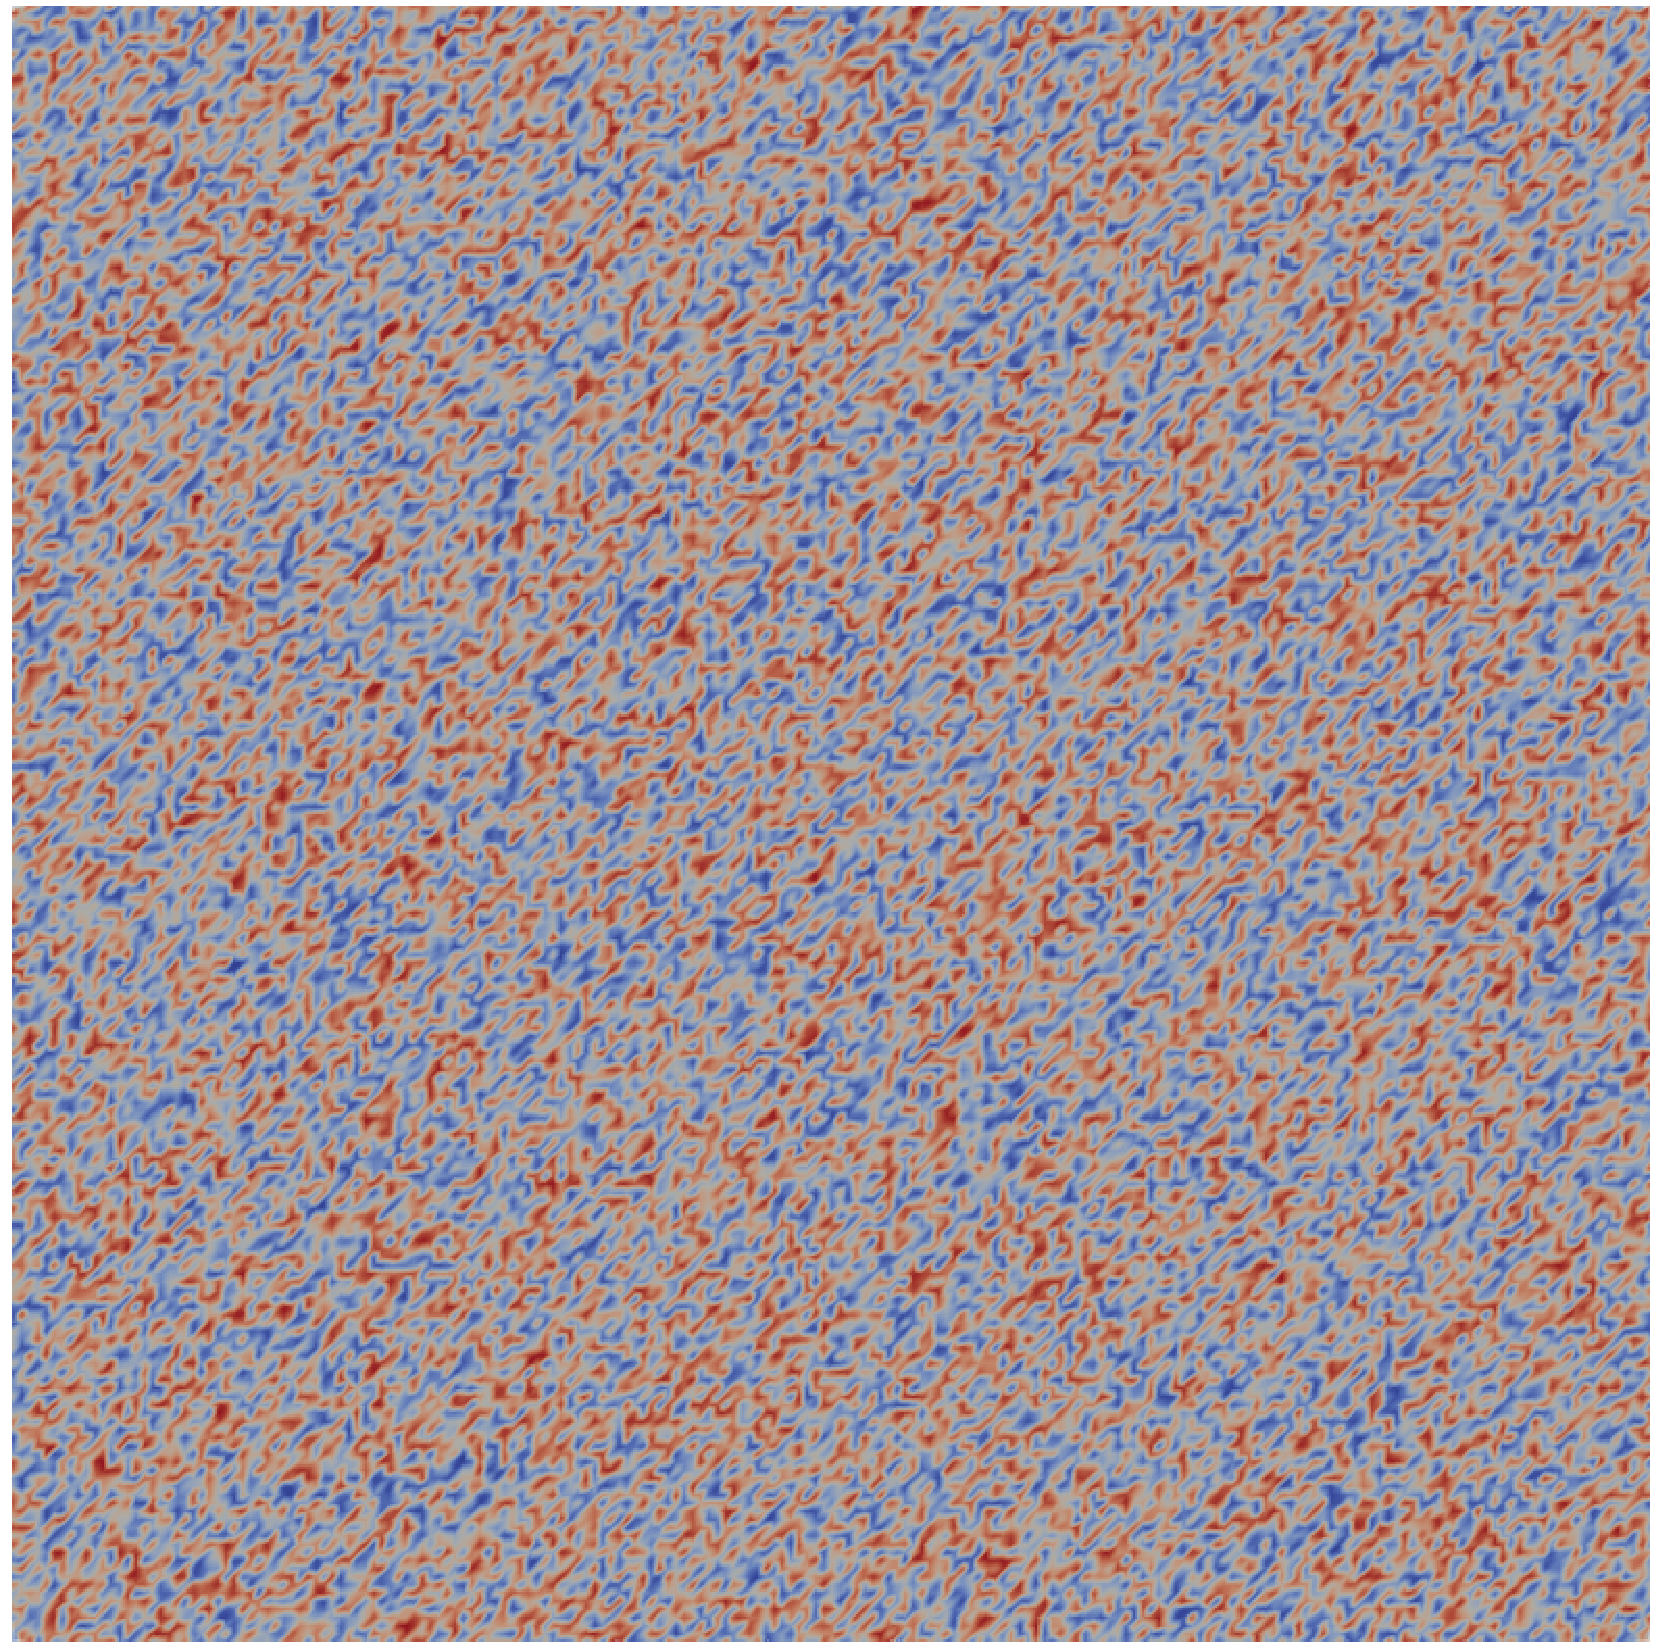
\includegraphics[width=0.95\textwidth]{Imagenes/Maxwell2D/Maxwell2D_sim/Imagenes/t_0}
        \caption{$t=0$}
    \end{subfigure}
    \begin{subfigure}[t]{0.45\textwidth}
        \centering
        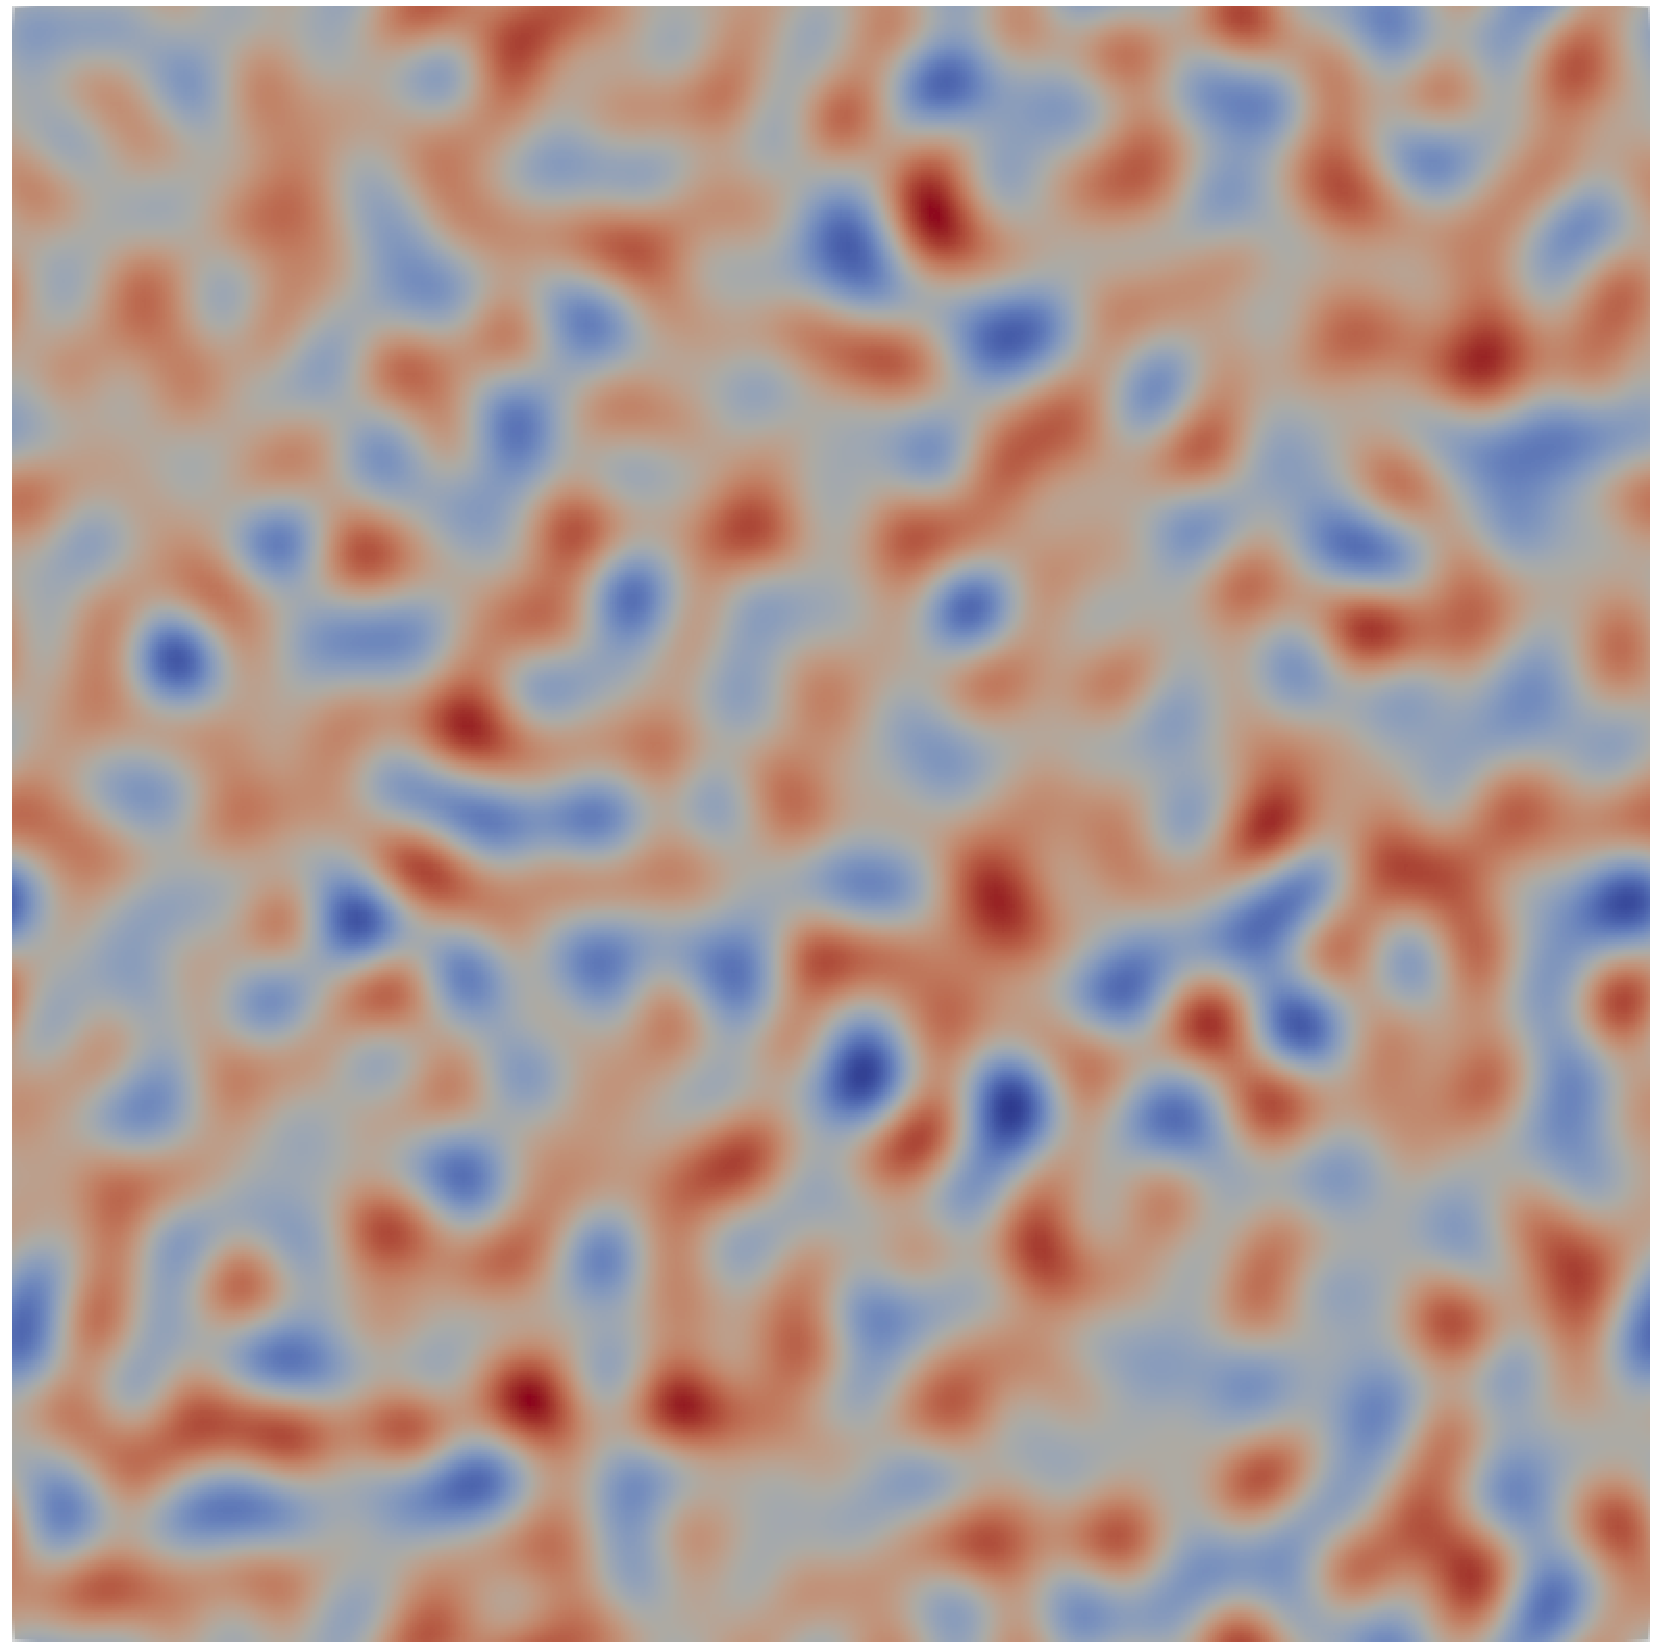
\includegraphics[width=0.95\textwidth]{Imagenes/Maxwell2D/Maxwell2D_sim/Imagenes/t_50}
        \caption{$t = 50$}
    \end{subfigure}
    \begin{subfigure}[t]{0.45\textwidth}
        \centering
        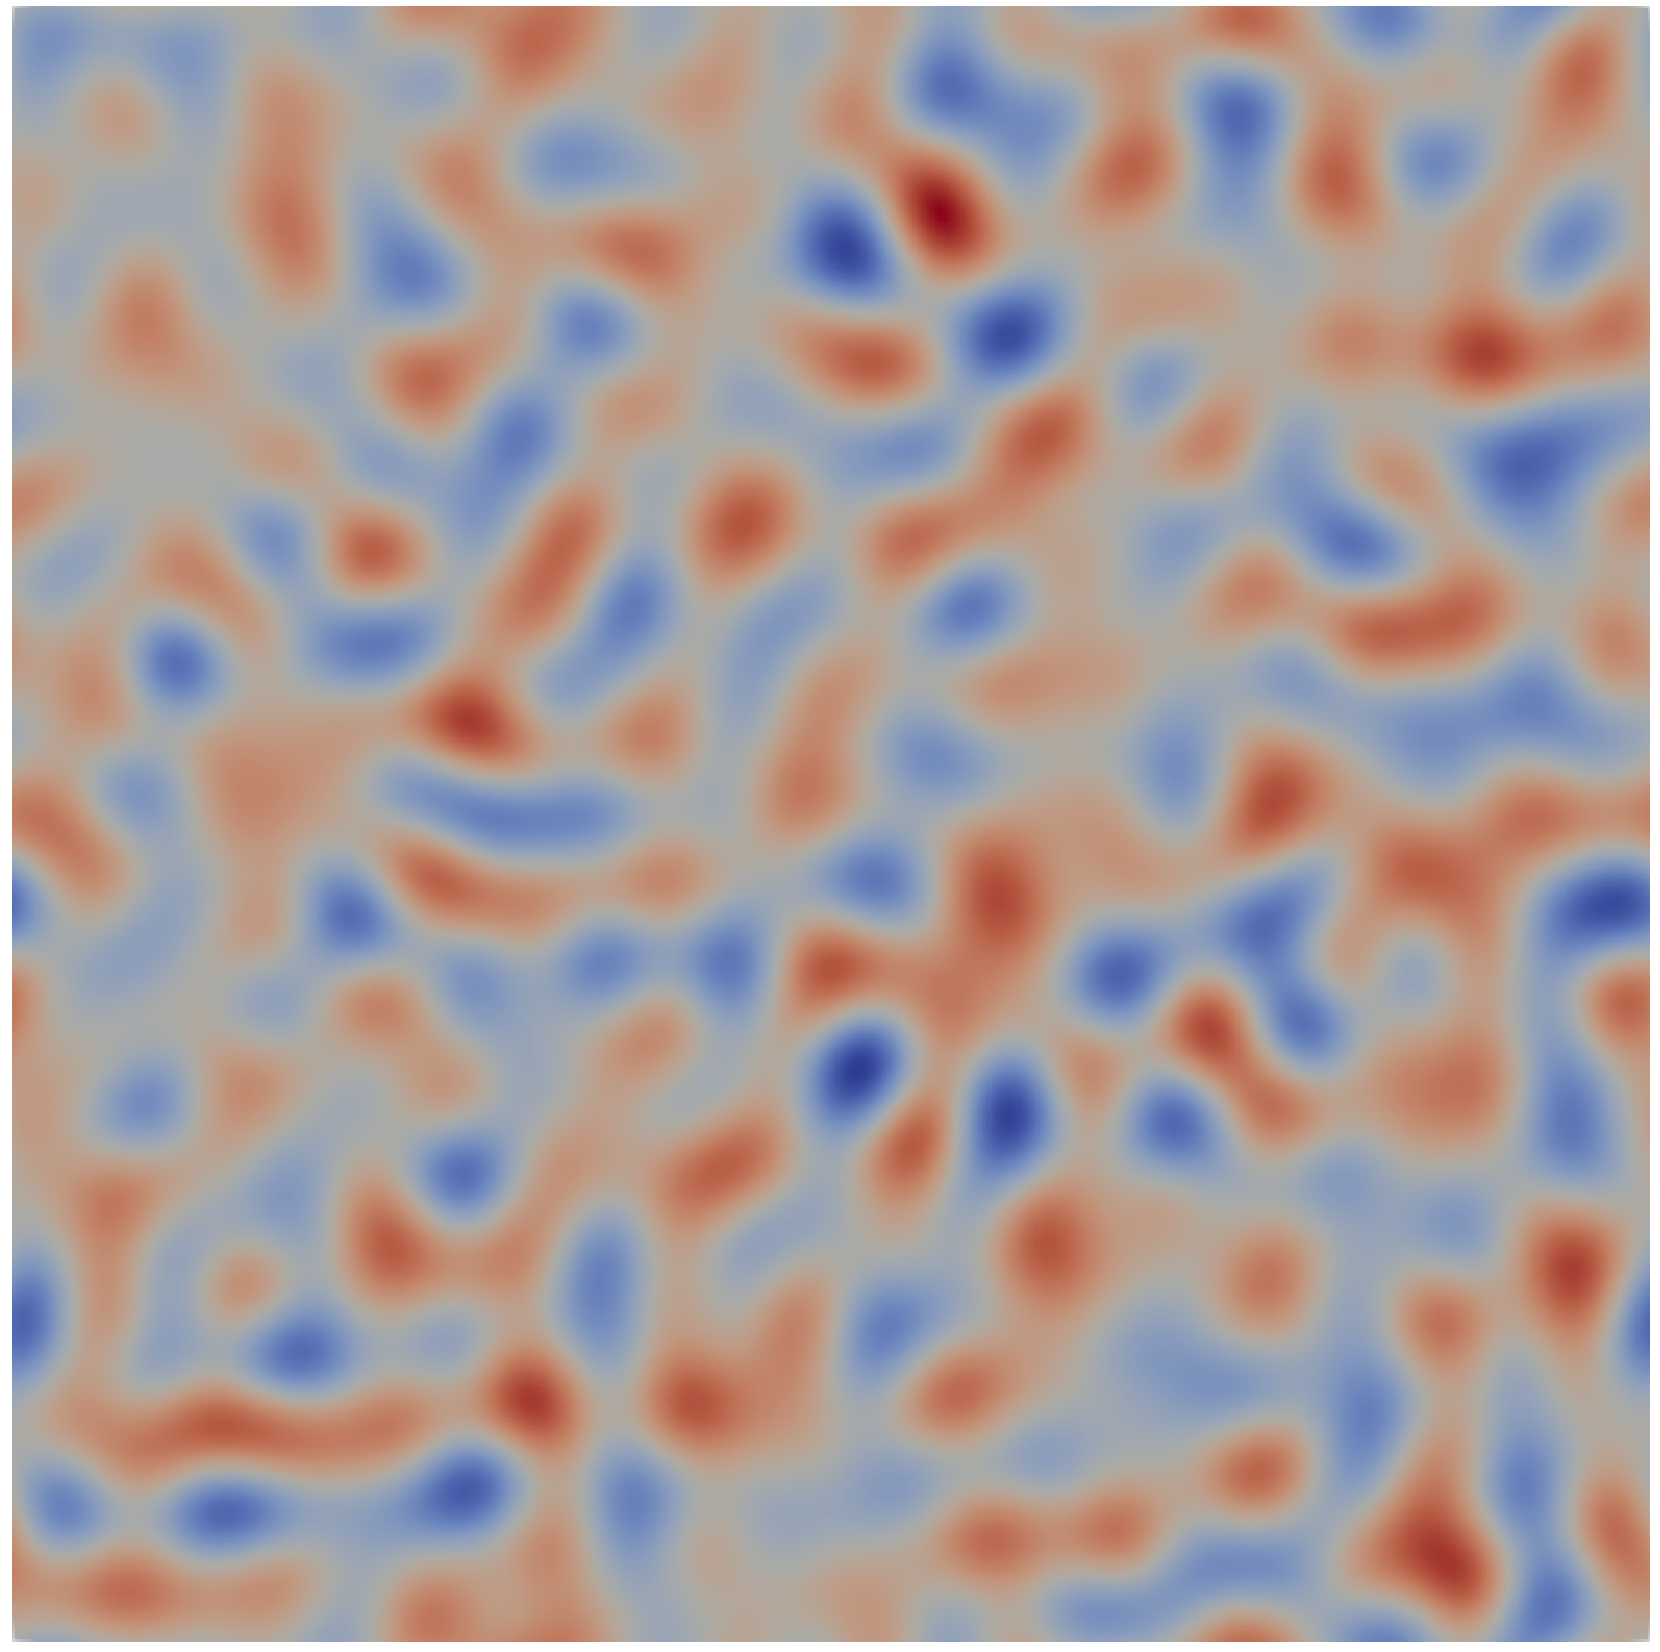
\includegraphics[width=0.95\textwidth]{Imagenes/Maxwell2D/Maxwell2D_sim/Imagenes/t_100}
        \caption{$t = 100$}
    \end{subfigure}    
    \begin{subfigure}[t]{0.45\textwidth}
        \centering
        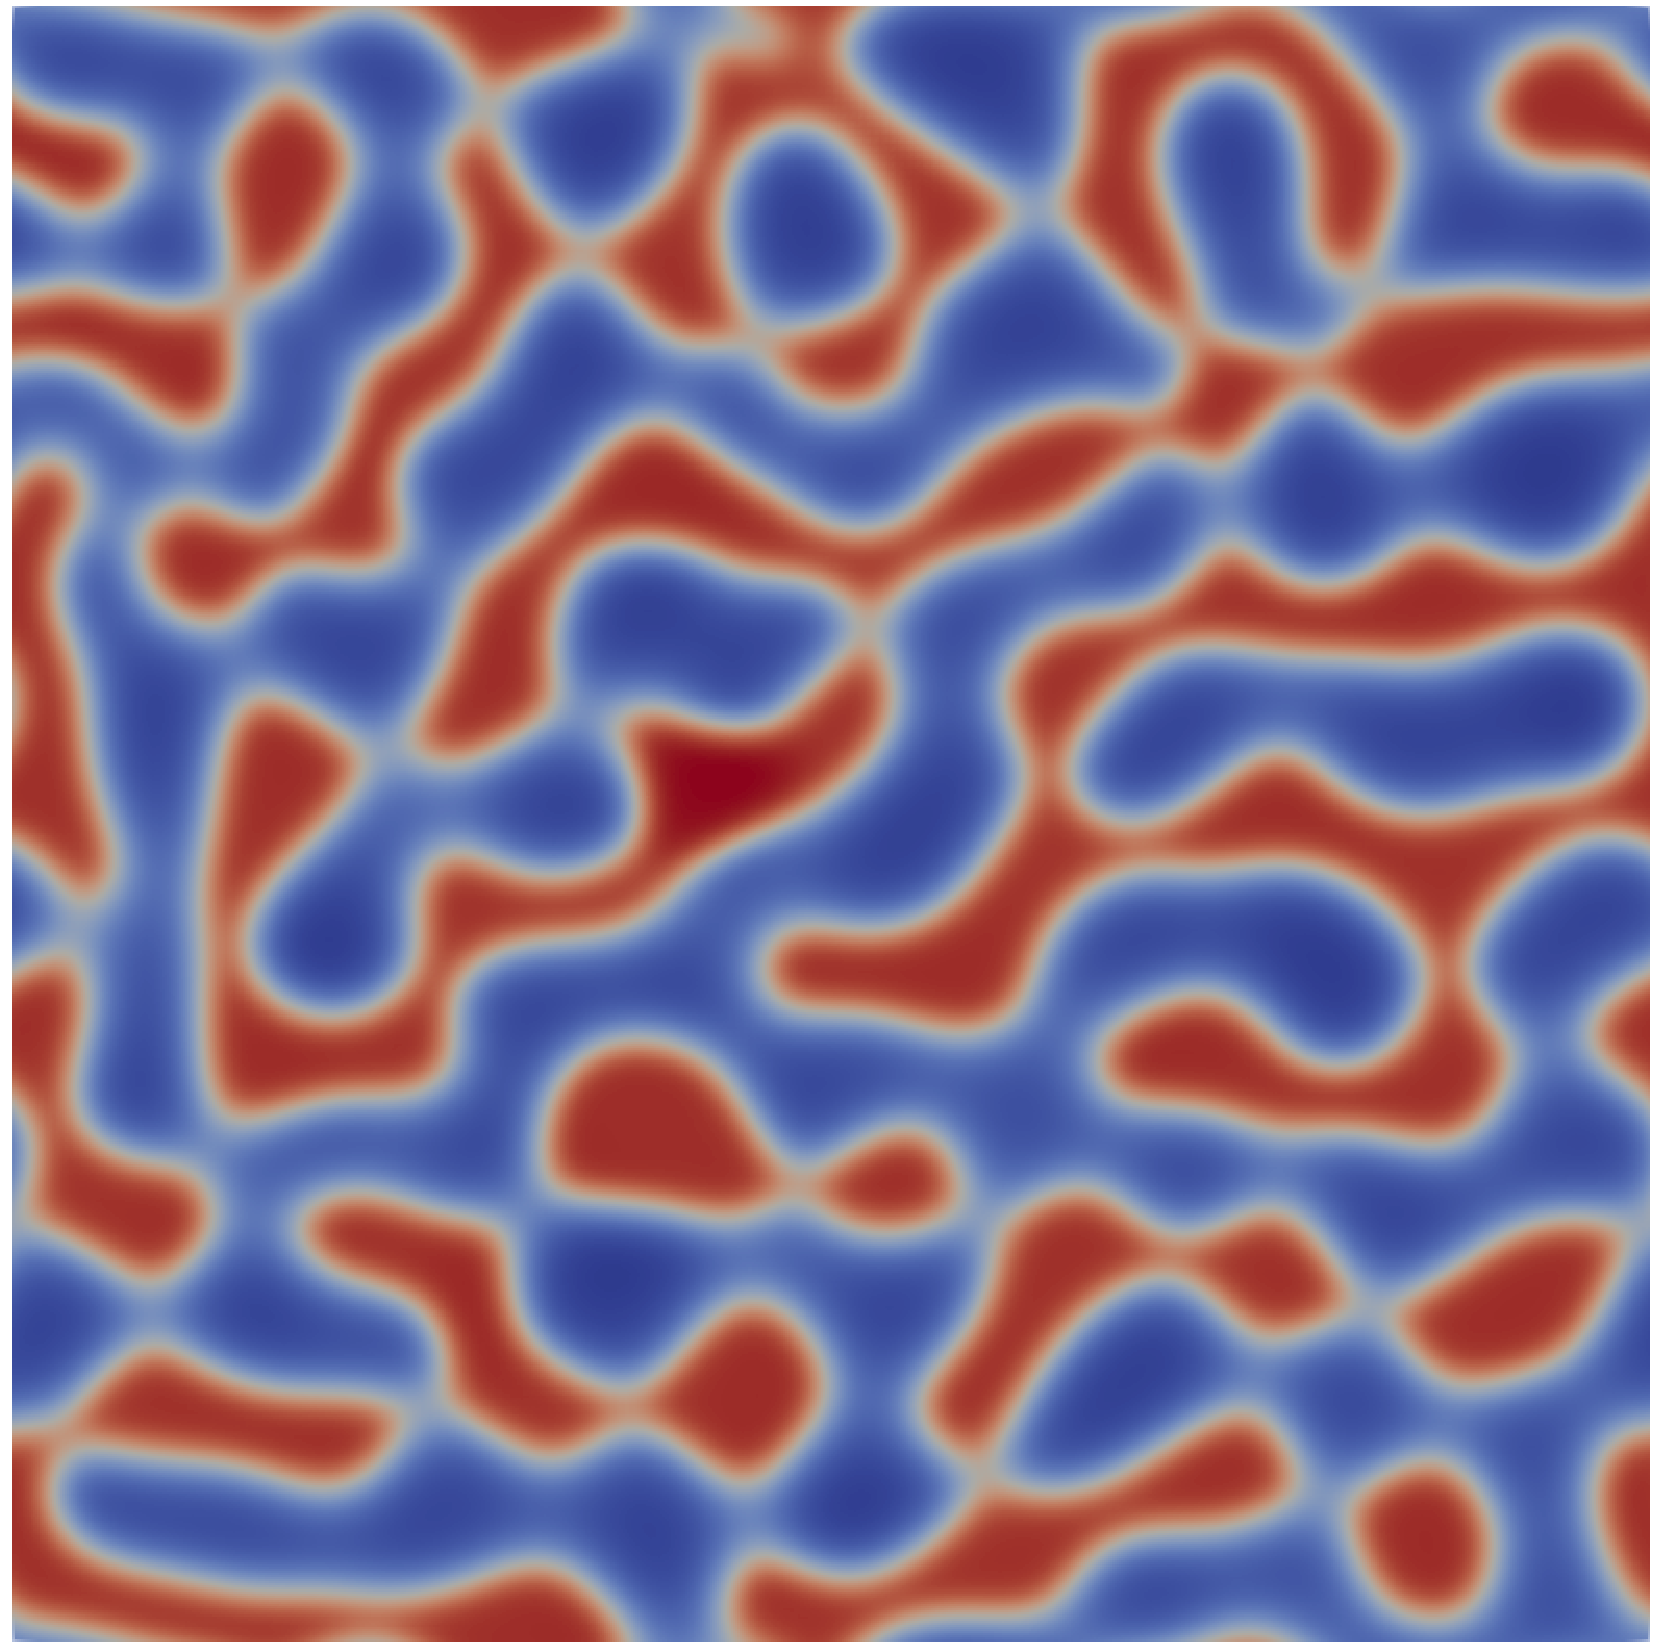
\includegraphics[width=0.95\textwidth]{Imagenes/Maxwell2D/Maxwell2D_sim/Imagenes/t_500}
        \caption{$t = 500$}
    \end{subfigure}    
    \begin{subfigure}[t]{0.45\textwidth}
        \centering
        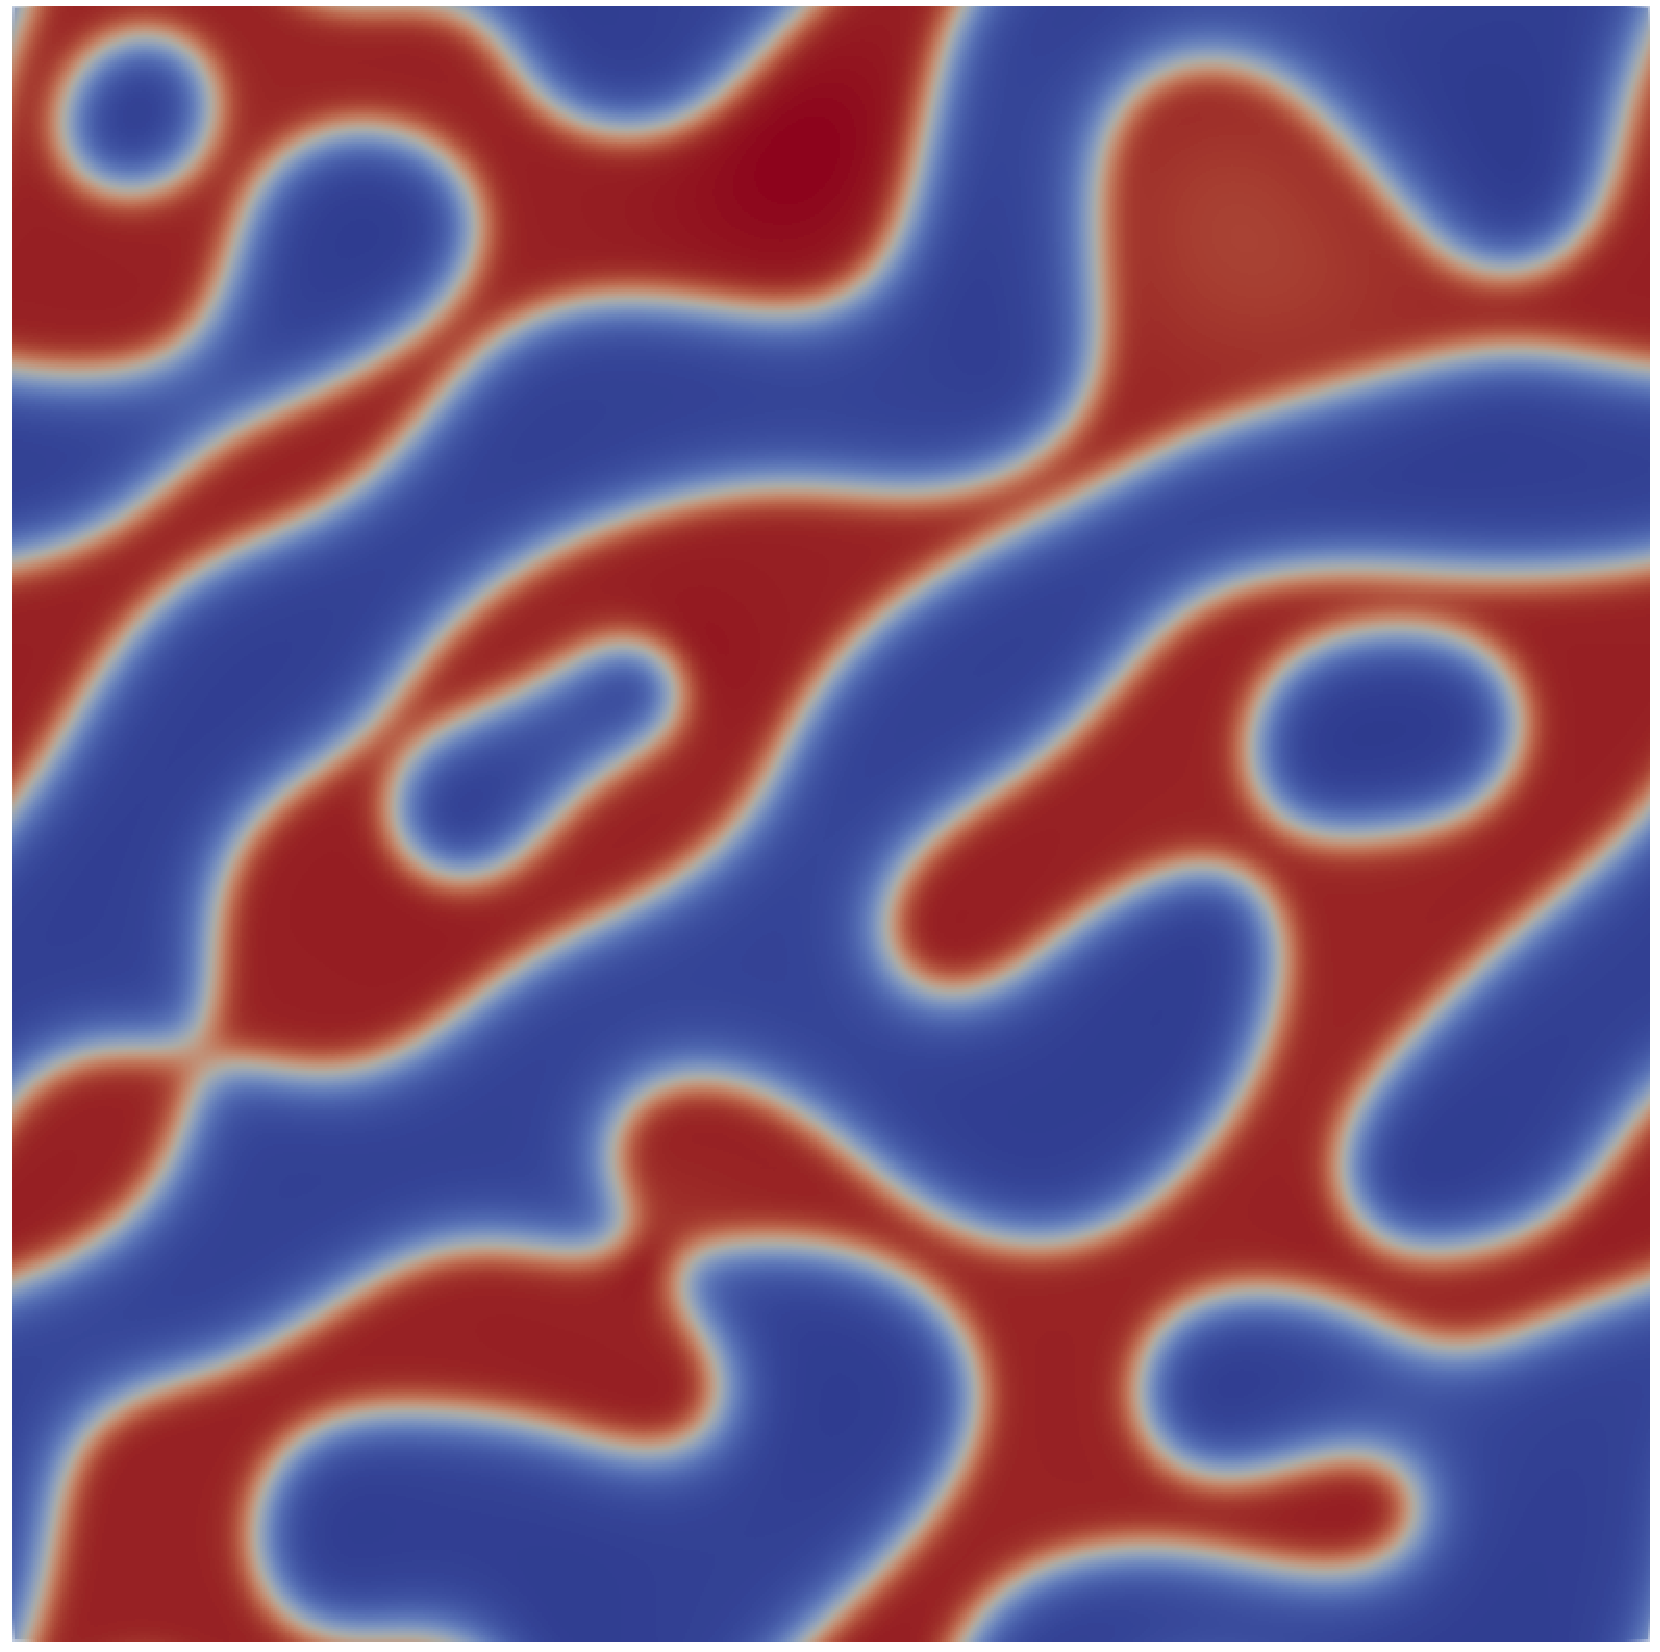
\includegraphics[width=0.95\textwidth]{Imagenes/Maxwell2D/Maxwell2D_sim/Imagenes/t_1000}
        \caption{$t = 1000$}
    \end{subfigure}
    \begin{subfigure}[t]{0.45\textwidth}
        \centering
        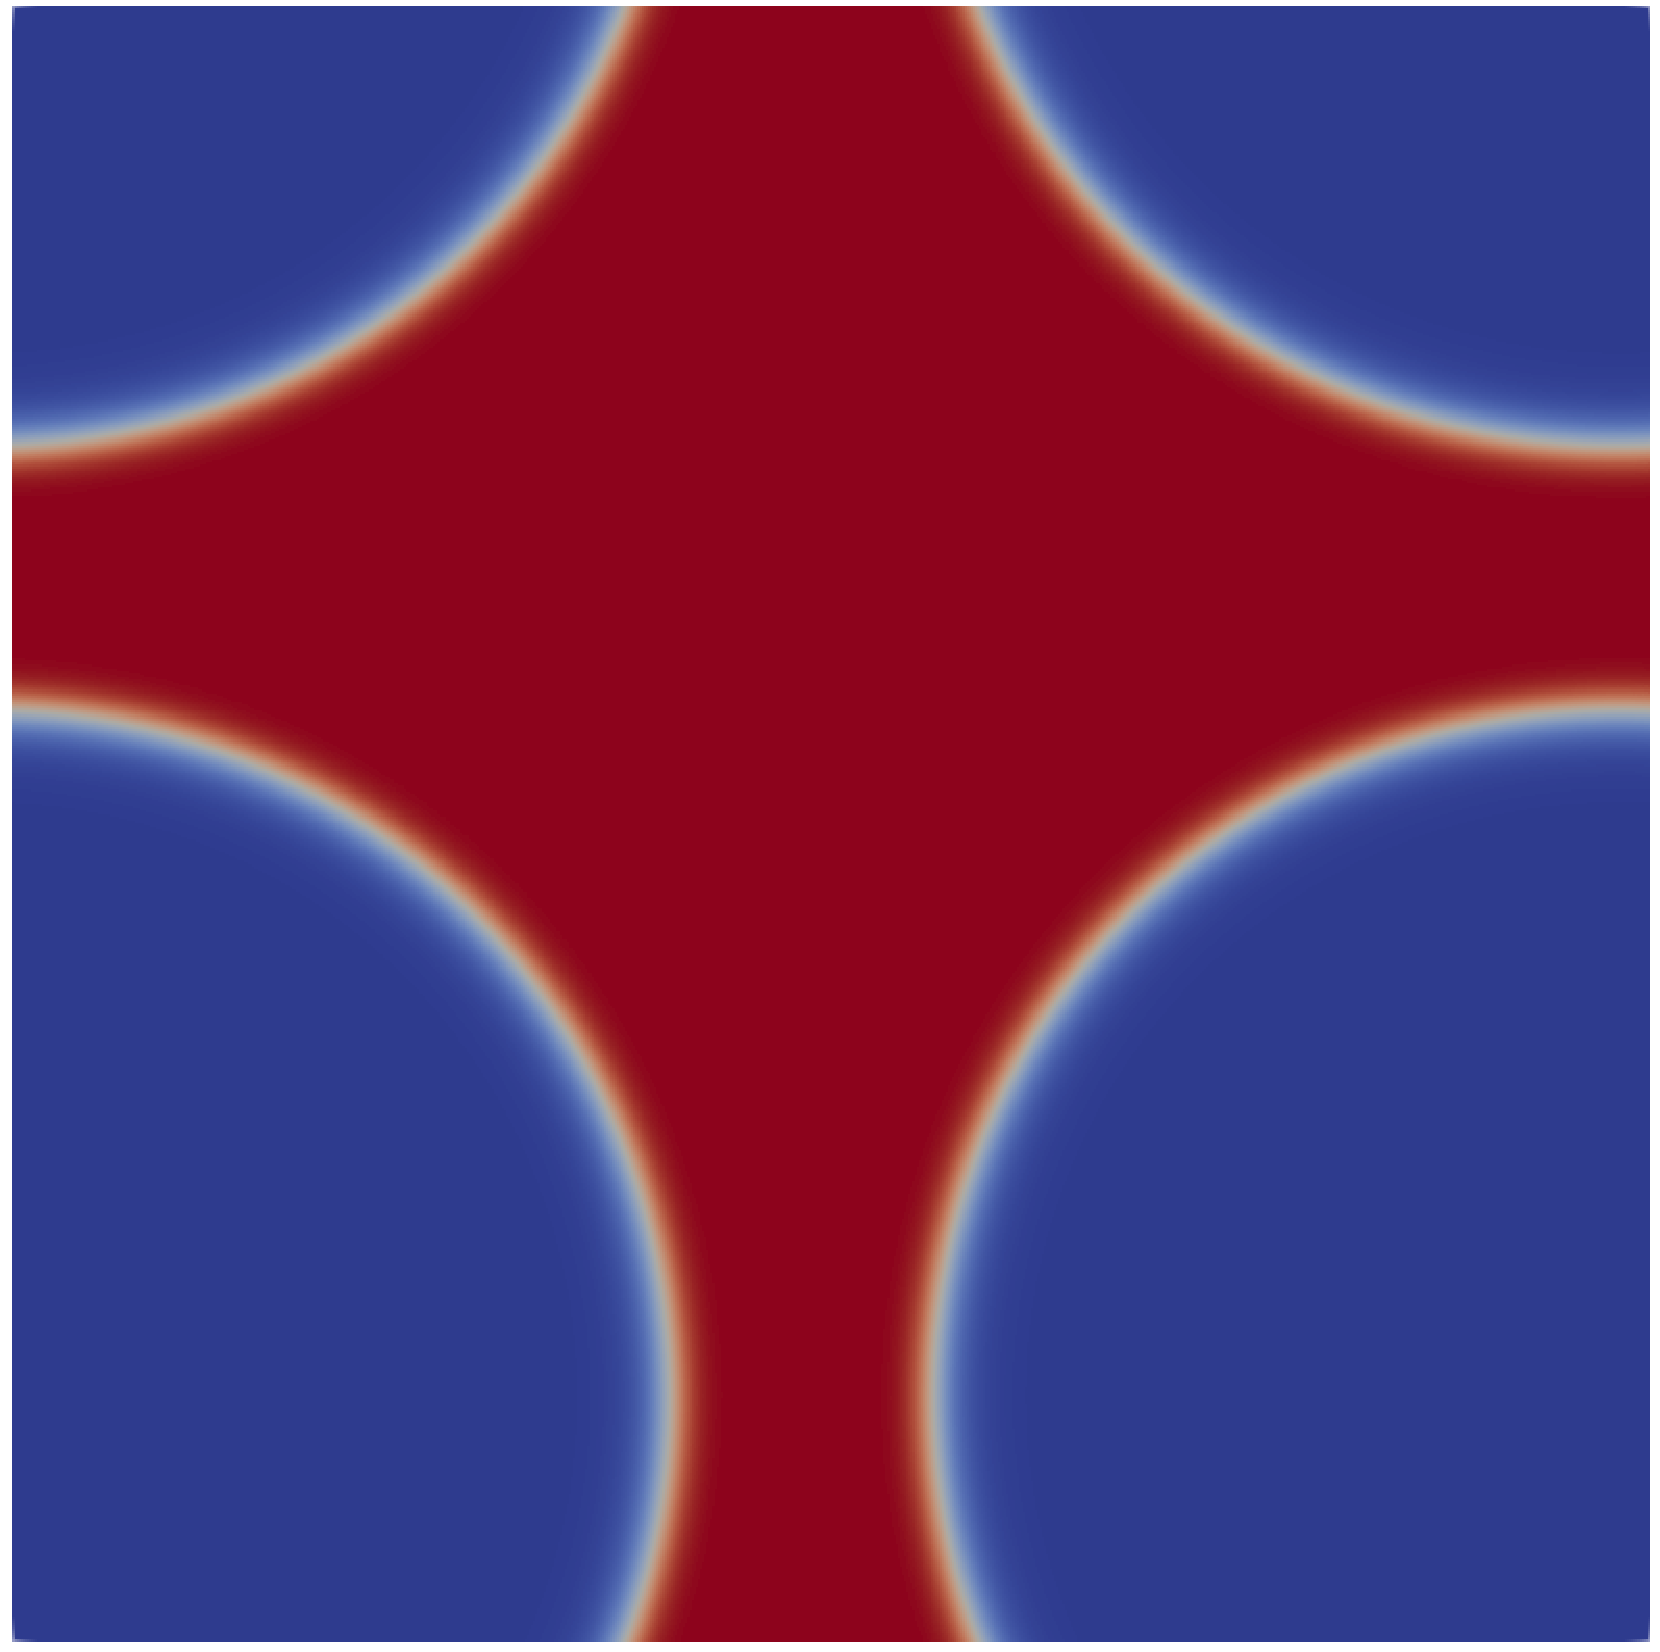
\includegraphics[width=0.95\textwidth]{Imagenes/Maxwell2D/Maxwell2D_sim/Imagenes/t_50000}
        \caption{$t = 50000$}
    \end{subfigure}        
    \caption{Evoluci\'on de una regi\'on bidimensional, peri\'odica, isot\'ermica y sin fuerzas externas, usada para verificar la regla de construcci\'on de Maxwell.}
    \label{fig:maxwell_2d}
\end{figure}
\FloatBarrier

Este problema de ejemplo resulta extremadamente \'util para evaluar el comportamiento del modelo de Li, en particular el efecto de la constante libre $\sigma$ sobre las densidades de coexistencia reproducidas. Para llevar a cabo esta compraraci\'on se simularon dominios peri\'odicos de $200\times 200$ u.g, incorporando la ecuaci\'on de estado de van der Waals con $a=0.5$ y $b=4$. En todos los casos se utilizaron las constantes $M=1$, $G=-1$, $R=1$, y los factores de relajaci\'on fueron fijados en $\tau_{\rho} = \tau_j=1$, $\tau_{e}^{-1}=\tau_{\zeta}^{-1}=\tau_{q}^{-1}=\tau_{\nu}^{-1}=1.1$. En la \fig{fig:maxwell_vdW} se observa que, de manera similar a lo mostrado en el trabajo original de Li \cite{li_lattice_2013} para la ecuaci\'on de Carnahan-Starling, el par\'ametro libre $\sigma$ puede ajustarse para lograr una reproducci\'on satisfactoria de la curva de coexistencia. En este caso, el uso de $\sigma=1/8$ conduce a densidades de coexistencia similares a las obtenidas mediante la regla de Maxwell, para temperaturas reducidas mayores que $0.5$. A partir de la \fig{fig:maxwell_vdW} tambi\'en es posible inferir que con la versi\'on original de un modelo \pp{} MRT, es decir con $\sigma=0$, queda limitado el rango de temperaturas para las cu\a'les s arregla satisfactoriamente la inconsistencia termodin\'amica.

\begin{figure}[ht]
	\centering
	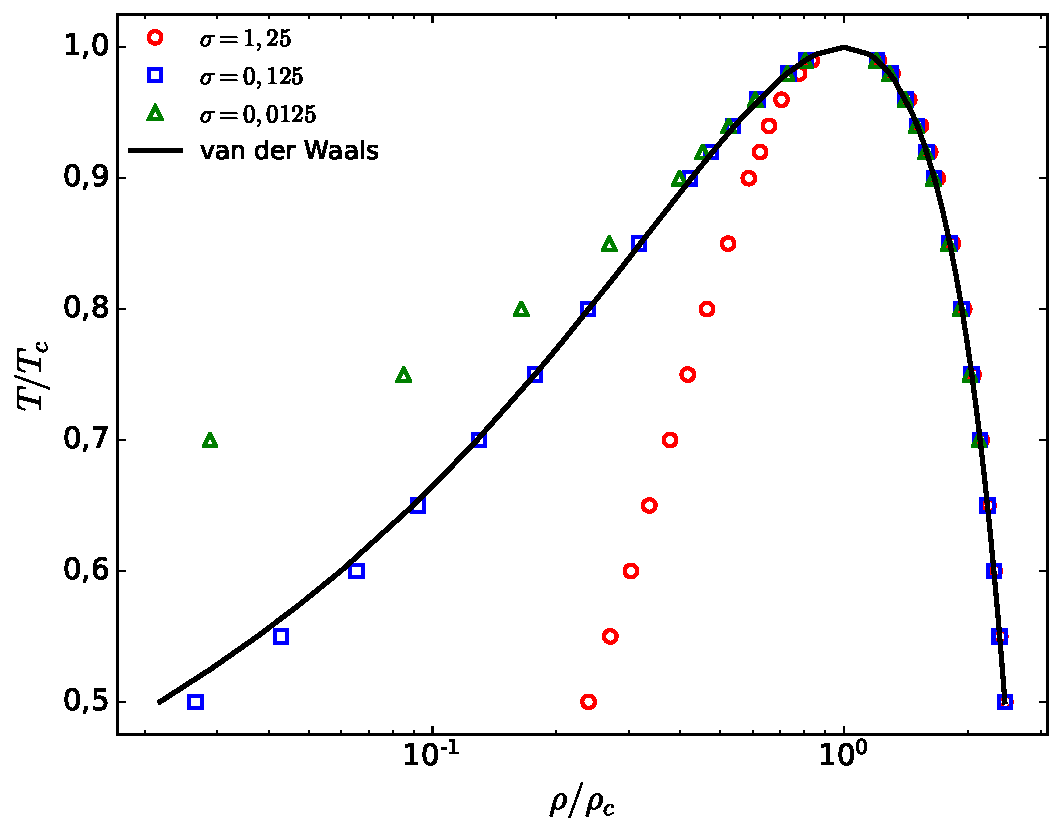
\includegraphics[width=0.75\textwidth]{Maxwell2D/Coexistencia/vdW_sigma}
	\caption{Densidades de coexistencia para la ecuaci\'on de estado de van der Waals, utilizando diferentes valores de $\sigma$. La l\'inea continua corresponde a la regla de construcci\'on de Maxwell.}
	\label{fig:maxwell_vdW}
\end{figure}

Es importante destacar que si no se observaron diferencias significativas en la reproducci\'on de la curva de coexistencia para distintos factores de relajaci\'on. Sin embargo, el valor de $\sigma$ m\'as adecuado est\'a vinculado a los valores de las constantes $a$ y $b$, como se muestra en la \fig{fig:maxwell_vdW_eos}

\begin{figure}[ht]
	\centering
	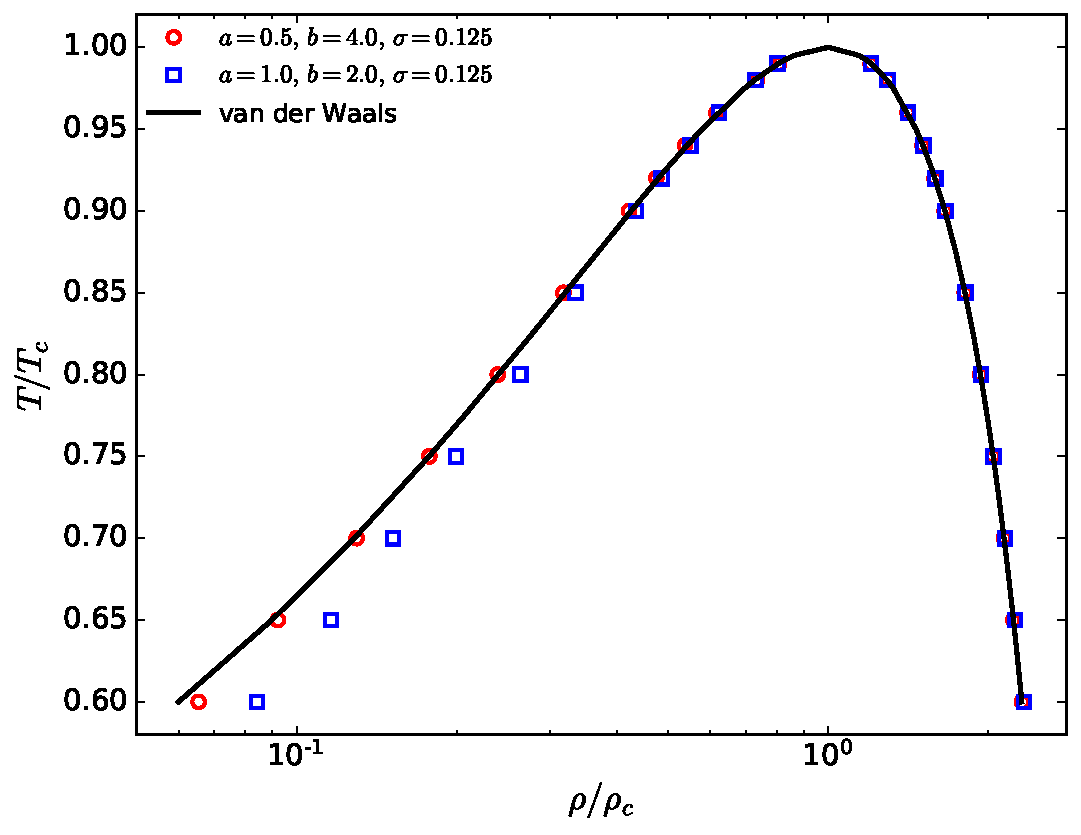
\includegraphics[width=0.75\textwidth]{Maxwell2D/Sigma_eos_const/vdW_sigma_eos}
	\caption{Densidades de coexistencia para la ecuaci\'on de estado de van der Waals, utilizando diferentes constantes para la ecuaci\'on de estado. La l\'inea continua corresponde a la regla de construcci\'on de Maxwell.}
	\label{fig:maxwell_vdW_eos}
\end{figure}


\subsection{Estratificaci\'on de un fluido van der Waals}

La validaci\'on de un m\'etodo num\'erico destinado a la resoluci\'on de flujo multif\'asico no es una tarea sencilla, ya que muchas veces no se cuenta con problemas o soluciones de referencia que sirvan como base de comparaci\'on. En el caso de lattice Boltzmann, tradicionalmente se ha utilizado una gran variedad de problemas como casos de validaci\'on; adem\'as de los ya mencionados, como medici\'on del per\'iodo de oscilaci\'on de droplets o estudio de impacto de droplets sobre superficies planas, es posible adicionar otros como el decaimiento de v\'ortices de Taylor \cite{guo_discrete_2002}, ondas de capilaridad \cite{mccracken_multiple-relaxation-time_2005} o inestabilidades de Rayleigh-Taylor \cite{li_additional_2012}. En estos casos, la figura de m\'erito de la comparaci\'on suele ser una magnitud global de la simulaci\'on, como la velocidad de avance de una interfase, o la amplitud y per\'iodo de una oscilaci\'on inducida. Si bien el seguimiento de estos par\'ametros es v\'alido para establecer una caracterizaci\'on de la precisi\'on del m\'etodo, en este proceso resulta dif\'icil de identificar, en un mismo problema, caracter\'isticas de una simulaci\'on propia de un modelo \pp{}: densidades de coexistencia, ancho de interfase, efecto de fuerzas volum\'etricas o resoluci\'on de grilla.

Esta necesidad de complementar la validaci\'on de un modelo \pp{} llev\'o a la adaptaci\'on y expansi\'on de una soluci\'on anal\'itica originalmente presentada por Berberan-Santos et al \cite{berberan-santos_liquidvapor_2002}, que permite determinar el perfil de densidad de un fluido regido por la ecuaci\'on de estado de van der Waals, dentro de una cavidad y bajo acci\'on de una fuerza gravitatoria.  Los primeros resultados de este an\'alisis fueron publicados oportunamente en el trabajo de Fogliatto et al \cite{fogliatto_simulation_2019}.

La idea detr\'as de este problema es conceptualmente sencilla. Si se tiene un fluido van der Waals dentro de un campo gravitacional uniforme, con gravedad en el sentido negativo de la coordenada $y$, entonces la distribuci\'on est\'atica de presi\'on satisface:
\begin{equation}
	\dfrac{dp}{dy} = -g\rho(y) = -MgC(y),
	\label{eq:p_hidrost}
\end{equation}
donde $M$ corresponde a la masa molar y $C=1/v$ a la concentraci\'on molar. Si la presi\'on del fluido est\'a asociada a la ecuaci\'on de estado de van der Waals
\begin{equation}
	p = \dfrac{RT}{v-b} - \dfrac{a}{v^2} = \dfrac{RT}{1/C-b} - aC^2,
\end{equation}
y se considera que la temperatura puede variar con la coordenada $y$, entonces la \eq{eq:p_hidrost} puede escribirse como
\begin{equation}
	\begin{array}{rcl}
		\dfrac{dp}{dy} &=& \dfrac{\partial p }{\partial C} \dfrac{\partial C}{\partial y}	 + \dfrac{\partial p}{\partial T}\dfrac{\partial T}{\partial y} \\[3mm]
		&=& \dfrac{\partial C}{\partial y}\left[ \dfrac{RT(1/C^2)- 2aC(1/C-b)^2}{(1/C-b)^2} \right] + \dfrac{\partial T}{\partial y}\left( \dfrac{R}{1/C-b}\right)
	\end{array}
	\label{eq:partial_p}
\end{equation}

Combinando las \eqs{eq:p_hidrost}{eq:partial_p} puede obtenerse una ecuaci\'on diferencial para la distribuci\'on de la concentraci\'on molar:
\begin{equation}
	\dfrac{\partial C}{\partial y} = -\left[ MgC + \dfrac{\partial T}{\partial y}\left( \dfrac{RC}{1-bC} \right) \right] \left[ \dfrac{RT}{(1-bC)^2} -2aC \right]^{-1}
	\label{eq:vdw_molar}
\end{equation} 

La \eq{eq:vdw_molar} corresponde a una ecuaci\'on diferencial ordinaria ordinaria y no lineal para la concentraci\'on molar, de modo que a trav\'es de su adecuada resoluci\'on es posible calcular la distribuci\'on de densidad dentro de la cavidad. 
La b\'usqueda de esta soluci\'on puede simplificarse si se hace uso de la ley de similaridad mostrada en la Secci\'on~\ref{sec:EOS}. En particular, es necesario introducir las variables adimensionales
\begin{equation}
	E_r = \dfrac{Mgy}{RT_c}, \qquad \rho_r=Cv_c=\dfrac{\rho}{\rho_c}, \qquad p_r=\dfrac{p}{p_c}, \qquad T_r = \dfrac{T}{T_c}, \qquad v_c = 3b
\end{equation}
donde $E_r$ se denota como energ\'ia gravitacional reducida. De esta forma, si se incorporan las variables adimensionales a la \eq{eq:vdw_molar}, es posible obtener una ecuaci\'on diferencial expresada \'unicamente en unidades reducidas:
\begin{equation}
	\dfrac{d\rho_r}{dE_r} = -\left[ \rho_r + \dfrac{dT_r}{dE_r} \left( \dfrac{\rho_r}{1-\rho_r/3} \right) \right]
\left[ \dfrac{T_r}{(1-\rho_r/3)^2} -\dfrac{9}{4}\rho_r \right]^{-1}
	\label{eq:vdw_column_red}
\end{equation}

La integraci\'on de la \eq{eq:vdw_column_red} debe realizarse a partir de la ubicaci\'on de la interfase, $E_r = E_{r_0}$, y requiere como condici\'on inicial a las densidades de coexistencia. De esta forma, la integraci\'on se realiza considerando $\rho_r(E_{r_0}) = \rho_{g_r}$ para $E_r > E_{r_0}$ y $\rho_r(E_{r_0}) = \rho_{l_r}$ para $E_r < E_{r_0}$. En el caso de la ecuaci\'on de  estado de van der Waals, la integral de la regla de construcci\'on de Maxwell puede resolverse de manera anal\'itica:
\begin{align}
	\int_{v_l}^{v_g} p \, \mbox{d}v' &= \int_{v_l}^{v_g} \left( \dfrac{RT}{v'-b} - \dfrac{a}{v'^2} \right) \mbox{d}v' \nonumber \\
		&= RT \ln \left( \dfrac{v_g - b}{v_l-b} \right) + a\left( \dfrac{1}{v_g} - \dfrac{1}{v_l} \right) \\
		&= p_0(v_g-v_l). \nonumber
		\label{eq:vdw_maxwell_analitica}
\end{align}

La \eq{eq:vdw_maxwell_analitica} tambi\'en puede escribirse usando variables reducidas:
\begin{equation}
	8T_r \ln \left( \dfrac{3/\rho_{g_r}-1}{3/\rho_{l_r}-1} \right) + 9(\rho_{g_r} - \rho_{l_r}) = 3p_{0_r} \left( \dfrac{1}{\rho_g} - \dfrac{1}{\rho_l} \right)
\end{equation}
donde $p_{0_r}$ corresponde a la presi\'on de saturaci\'on reducida. Es particular, si se expresa a la ecuaci\'on de estado de van der Waals en unidades reducidas:
\begin{equation}
 p_r = \dfrac{8 T_r}{3/\rho_r-1} - 3\rho_r,
\end{equation}
entonces puede usarse la igualdad $p_r(\rho_{g_r}) = p_r(\rho_{r_gl})$ para obtener una relaci\'on entre la temperatura reducida y las densidades de coexistencia:
\begin{equation}
	T_r = \dfrac{1}{8}(\rho_{l_r}+\rho_{g_r})(3-\rho_{l_r})(3-\rho_{g_r})
	\label{eq:tr_maxwell}
\end{equation}

Usando esta expresi\'on de $T_r$ para reescribir a la presi\'on de saturaci\'on
\begin{equation}
	p_{r_0} = p_r(\rho_{g_r}) = \rho_{g_r} \rho_{l_r} ( 3 - \rho_{l_r} - \rho_{g_r} ),
\end{equation}
entonces finalmente puede escribirse el resultado de la integral de la regla de construcci\'on de Maxwell en unidades reducidas como:
\begin{equation}
	\left( \dfrac{3/\rho_{g_r}-1}{3/\rho_{l_r}-1} \right) = \dfrac{\rho_{l_r} - \rho_{g_r}}{\rho_{l_r} + \rho_{g_r}}\left( \dfrac{3}{3-\rho_{l_r}} + \dfrac{3}{3-\rho_{g_r}} \right)
	\label{eq:rhor_maxwell}
\end{equation}

De esta manera, las \eqs{eq:tr_maxwell}{eq:rhor_maxwell} constituyen un sistema de ecuaciones no lineal que puede ser utilizado para encontrar las densidades de coexistencia $\rho_{g_r}$ y $\rho_{g_r}$ para una temperatura $T_r$.

La resoluci\'on de la distribuci\'on de densidad dentro de una cavidad debe cerrarse con un mecanismo para calcular la posici\'on de la interfase, el cual puede obtenerse a partir de la conservaci\'on de masa inicial de la cavidad:
\begin{equation}
	\begin{gathered}
		\int_{0}^{h_0} C_l(y') \, \mbox{d}y' + \int_{h_0}^{H} C_g(y') \, \mbox{d}y' = \bar{C}H ,\\[3mm]
		\int_{0}^{E_{r_0}} \rho_{l_r} (E'_r) \, \mbox{d}E'_r + \int_{E_{r_0}}^{E_{r_m}} \rho_{g_r}(E'_r) \, \mbox{d}E'_r = \bar{\rho_r}E_{r_m}, \\
	\end{gathered}
	\label{eq:masa_maxwell}
\end{equation}
donde $\bar{C}$ y $\bar{\rho_r}$ denotan a los valores promedio de concentraci\'on molar y densidad reducida respectivamente. En resumen, el conjunto de ecuaciones (\ref{eq:vdw_column_red}), (\ref{eq:tr_maxwell}), (\ref{eq:rhor_maxwell}) y (\ref{eq:masa_maxwell}) permite determinar, de manera num\'erica, c\'omo es la distribuci\'on de densidad para un fluido van der Waals dentro de una cavidad  bajo acci\'on de la gravedad. En este caso, se asume que ambas fases quedan claramente separadas por una interfase de espesor nulo, y que la temperatura en el interior del fluido sigue una distribuci\'on arbitraria, es decir, independiente de la densidad.  Esta \'ultima hip\'otesis en general no es v\'alida, pero aporta cierto grado de flexibilidad a la soluci\'on anal\'itica, y resulta de gran utilidad para evaluar el desempe\~no de un modelo \pp{}. Tomando en cuenta estas caracter\'isticas, el algoritmo implementado para encontrar la distribuci\'on de densidad queda descripto por los siguientes pasos:

\begin{enumerate}

\item Selecci\'on de una discretizaci\'on inicial $\Delta_0$ para el intervalo $[0.E_{r_m}]$.

\item Determinaci\'on de perfiles iniciales para la temperatura y densidad reducida. La distribuci\'on de temperatura elegida no cambia con los pasos siguientes.

\item Elecci\'on de una posici\'on inicial para la interfase, $E_{r_0}^{(0)}$.

\item \label{itm:rhor_tr} C\'alculo de las densidades de coexistencia para $T_r(E_{r_0}^{(0)})$ usando las \eqs{eq:tr_maxwell}{eq:rhor_maxwell}.

\item Integraci\'on de la \eq{eq:rhor_maxwell} hacia ambos lados de la interfase usando esquemas de diferencias finitas adelantadas de segundo orden. Espec\'ificamente, si la interfase se encuentra en la posici\'on $E_{r_0}^{(k)}$, donde el supra\'indice $k$ corresponde al n\'umero de iteraci\'on, ,entonces es necesario integrar la \eq{eq:rhor_maxwell} entre $E_{r_0}^{(k)}$ y $E_{r_m}$ usando
\begin{equation}
	\rho_r(E_{r_j} + 2\Delta) = -3\rho_r(E_{r_j}) + 4\rho_r(E_{r_j} + \Delta) - 2\Delta \left.\dfrac{d \rho_r}{d E_r} \right|_{E_{r_j}},
\end{equation}
donde se define la posici\'on $E_{r_j} = E_{r_0}^{(k)} + j\Delta$ y $\Delta$ se calcula mediante
\begin{equation}
	\Delta = \dfrac{E_{r_{max}} - E_{r_0}^{(k)}}{\mbox{int} \left( \dfrac{E_{r_{max}} - E_{r_0}^{(k)}}{\Delta_0} \right)}.
\end{equation}

De esta forma, tomando como condici\'on inicial a a $\rho_r(E_{r_0}^{(k)}) = \rho_{g_r}(E_{r_0}^{(k)})$, puede calcularse la densidad de la fase gaseosa en $\mbox{int}[ (E_{r_{max}} - E_{r_0}^{(k)} )/\Delta_0 ]$ puntos. El procedimiento es similar para la fase l\'iquida, es decir, $E_r \in [0,E_{r_0}^{(k)}]$.

\item C\'alculo del exceso (o defecto) de masa usando la \eq{eq:masa_maxwell}. Si la igualdad no se cumple, debe reubicarse a la interfase en una nueva posici\'on $E_{r_0}^{(k+1)} < E_{r_0}^{(k)}$ si existe exceso de masa, o $E_{r_0}^{(k+1)} > E_{r_0}^{(k)}$ si hay defecto de la misma. La determinaci\'on de esta ubicaci\'on se hace mediante la t\'ecnica de bisecci\'on, es decir, conservando las posiciones l\'imites admisibles a cada lado de la interfase (obtenidas de las iteraciones previas), y eligiendo el punto medio entre la posici\'on actual y el l\'imite correspondiente.

\item Repetici\'on a partir del punto \ref{itm:rhor_tr}, calculando las densidades de coexistencia para $T_r(E_{r_0}^{(k+1)})$ e iterando hasta que la posici\'on de la interfase converja con una tolerancia preestablecida.

\end{enumerate}


La distribuci\'on de densidad en una cavidad constituye un excelente caso de prueba para un modelo \pp{} con ecuaci\'on de estado de van der Waals, ya que no s\'olo permite verificar la correcta reproducci\'on de la curva de coexistencia, sino que permite visualizar el efecto de la inclusi\'on de fuerza gravitatoria, temperatura no uniforme y resoluci\'on de grilla. Para representar este problema con lattice Boltzmann se defini\'o una cavidad bidimensional de $L=3$ unidades de grilla en la direcci\'on horizontal ($x$) y $H$ unidades de grilla en la direcci\'on vertical ($y$), como se muestra esquem\'aticamente en la \fig{fig:vdWColumn_cavidad}. Para este problema se utiliz\'o una condici\'on de contorno per\'odica en la direcci\'on $x$, y el esquema de no deslizamiento de Zou y He \cite{zou_pressure_1997} en las caras restantes. En todos los casos mostrados en el presente Cap\'itulo, la temperatura en las caras superior e inferior se fij\'o en $T_t$ y $T_b$ respectivamente, con una distribuci\'on lineal en el interior de la cavidad. Por otro lado, salvo que se indique expl\'icitamente lo cotrario, en todos los casos se utilizaron las constantes $M=1$, $G=-1$, $R=1$, $a=0.5$, $b=4$, y los factores de relajaci\'on fueron fijados en $\tau_{\rho} = \tau_j=1$, $\tau_{e}^{-1}=\tau_{\zeta}^{-1}=\tau_{q}^{-1}=\tau_{\nu}^{-1}=1.1$. Adem\'as, considerando los resultados de las pruebas de construcci\'on de Maxwell, se emple\'o en todos los casos $\sigma = 0.125$.

\begin{figure}[ht]
	\centering
	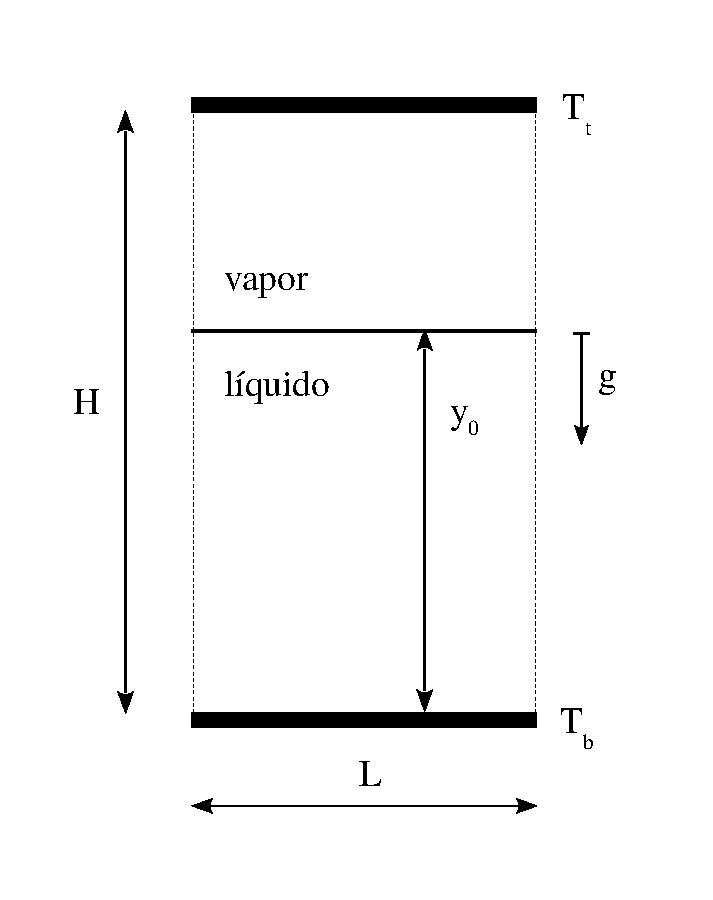
\includegraphics[width=0.6\textwidth]{vdWColumn/cavidad}
	\caption{Esquema del dominio empleado las simulaciones de un fluido van der Waals dentro de una cavidad.}
	\label{fig:vdWColumn_cavidad}
\end{figure}

Siguiendo un procedimiento similar al empleado en los problemas de construcci\'on de Maxwell, las simulaciones de inicializaron con una distribuci\'on de densidad perturbada aleatoriamente en $\pm1\%$ alrededor de un valor elegido, y en este caso se dejaron evolucionar hasta alcanzar un estado estacionario. Por otro lado, el valor de $g$ empleado en el t\'ermino de fuerza volum\'etrica se determin\'o a partir del par\'ametro adimensional $E_{r_{max}} = E_r(H)$.

En una primera prueba num\'erica, se utiliz\'o una cavidad con $H=300$, $E_r(H)=10^{-3}$, temperatura uniforme ($T_t = T_b = T_r$) y una densidad inicial (perturbada) igual a la cr\'tica, es decir $\rho_r=1$ . En la \fig{fig:vdWColumn_evolucion} se muestra, a modo de ejemplo, la distribuci\'on de densidad en una cavidad con $T_r=0.99$ para diferentes instantes de tiempo. Como puede observarse, despu\'es del instante inicial se produce una r\'apida separaci\'on de fases en  bandas horizontales. Como es esperable a partir del balance hidrost\'atico, despu\'es de un tiempo de simulaci\'on suficiente, la fase l\'iquida ocupa la parte inferior del dominio, mientras que la densidad es uniforme a lo largo de la coordenada horizontal.

\begin{figure}[ht]
	\centering
	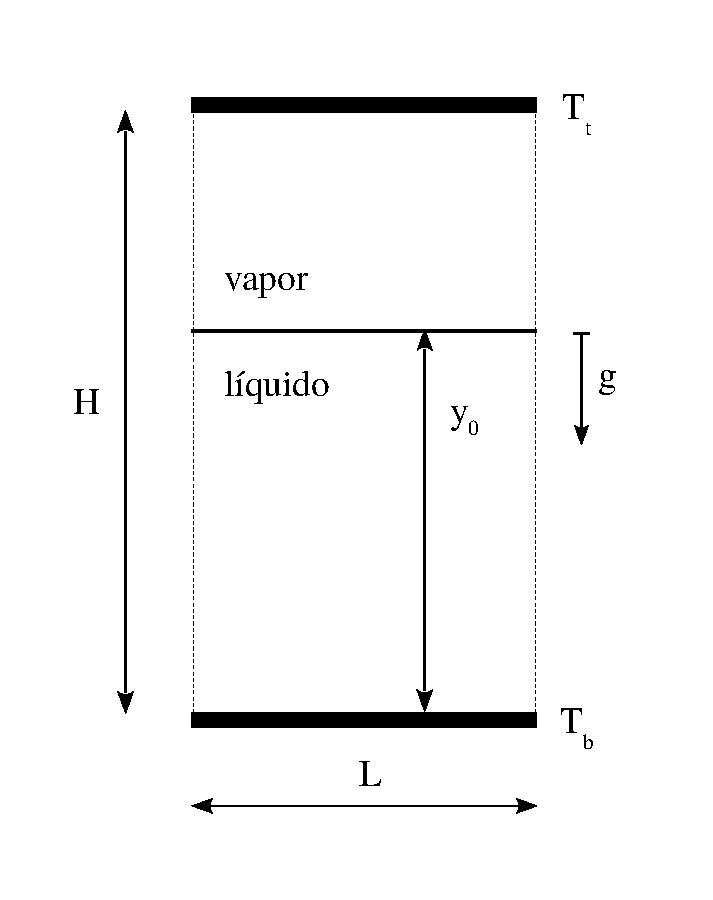
\includegraphics[width=0.6\textwidth]{vdWColumn/cavidad}
	\caption{Evoluci\'on}
	\label{fig:vdWColumn_evolucion}
\end{figure}

En la \fig{fig:vdWColumn_rhor_tuniform} se muestran los perfiles de densidad reducida sobre la coordenada vertical, expresada en unidades adimensionales como $y/H = E_r/E_r(H)$. Los perfiles corresponden al resultado de simulaciones con lattice Boltzmann para diferentes temperaturas, y se muestran junto con los calculados usando la expresi\'on anal\'itica. Como puede observarse, el modelo \pp{} de Li at al. con $\sigma=0.125$ es capaz de reproducir satisfactoriamente el perfil de densidad en el seno de cada fase, de modo que no se observan efectos apreciables de la fuerza volum\'etrica en la capacidad de corregir la inconsistencia termoden\'amica. Por otro lado, se observa que el modelo genera una variaci\'on de densidad continua a trav\'es de la interfase, y en estos casos, en d\'onde se mantienen todas las constantes de simulaci\'on salvo la temperatura del dominio, el espesor de esta interfase disminuye con la temperatura de la cavidad.

\begin{figure}[ht]
	\centering
	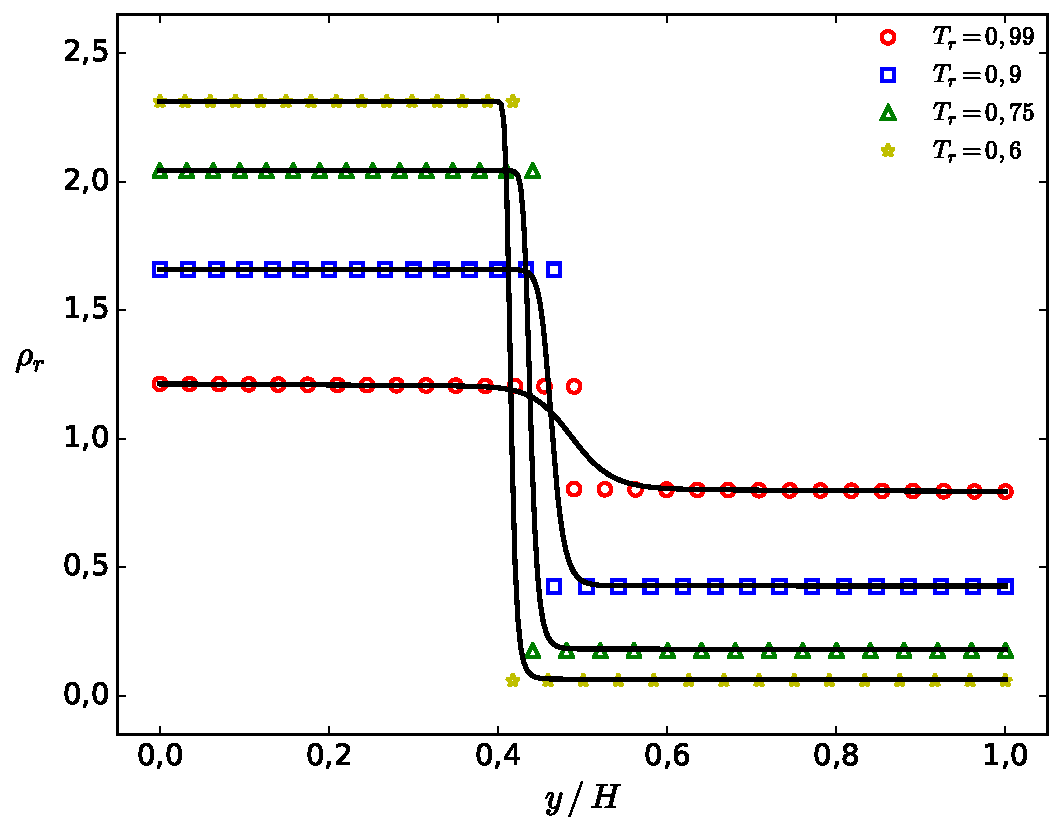
\includegraphics[width=0.75\textwidth]{vdWColumn/TUniform/rhor_vdWcolumn_Tuniform}
	\caption{Distribuci\'on espacial de densidad en una cavidad con fuerza gravitacional dada por $E_r(H)=10^{-3}$. Las l\'ineas continuas corresponden a simulaciones de lattice Boltzmann con $\sigma=0.125$, mientras que los puntos representan los valores obtenidos con la expresi\'on anal\'itica.}
	\label{fig:vdWColumn_rhor_tuniform}
\end{figure}

El an\'alisis de la distribuci\'on de densidad puede extenderse al uso de diferentes condiciones iniciales, como la incorporaci\'on de un fluido con distinta densidad promedio. En la \fig{fig:vdWColumn_frac_volumen} se muestra la dependencia de la posici\'on de la interfase (equivalente a fracci\'on de l\'iquido) con la temperatura de la cavidad. En el caso en que la densidad promedio sea igual a la cr\'itica ($\rho_r=1$), las fracciones de l\'iquido y vapor tienden a igualarse a medida que la temperatura se acerca a su valor cr\'itico. Si la densidad promedio es supercr\'itica ($\rho_r > 1$), el volumen de vapor tiende a cero a medida que la temperatura de la cavidad crece, de modo que se observa una temperatura l\'imite a partir de la cual se observa s\'olo una fase l\'iquida. Por otro lado, este comportamiento se invierte para una densidad inicial subcr\'itica ($\rho_r < 1$), por lo que la fracci\'on de fase l\'iquida tiende a cero con el incremento de temperatura. Como se observa en la \fig{fig:vdWColumn_frac_volumen}, este comportamiento predicho por la soluci\'on anal\'itica es reproducido correctamente por el modelo \pp{}.

\begin{figure}[ht]
	\centering
	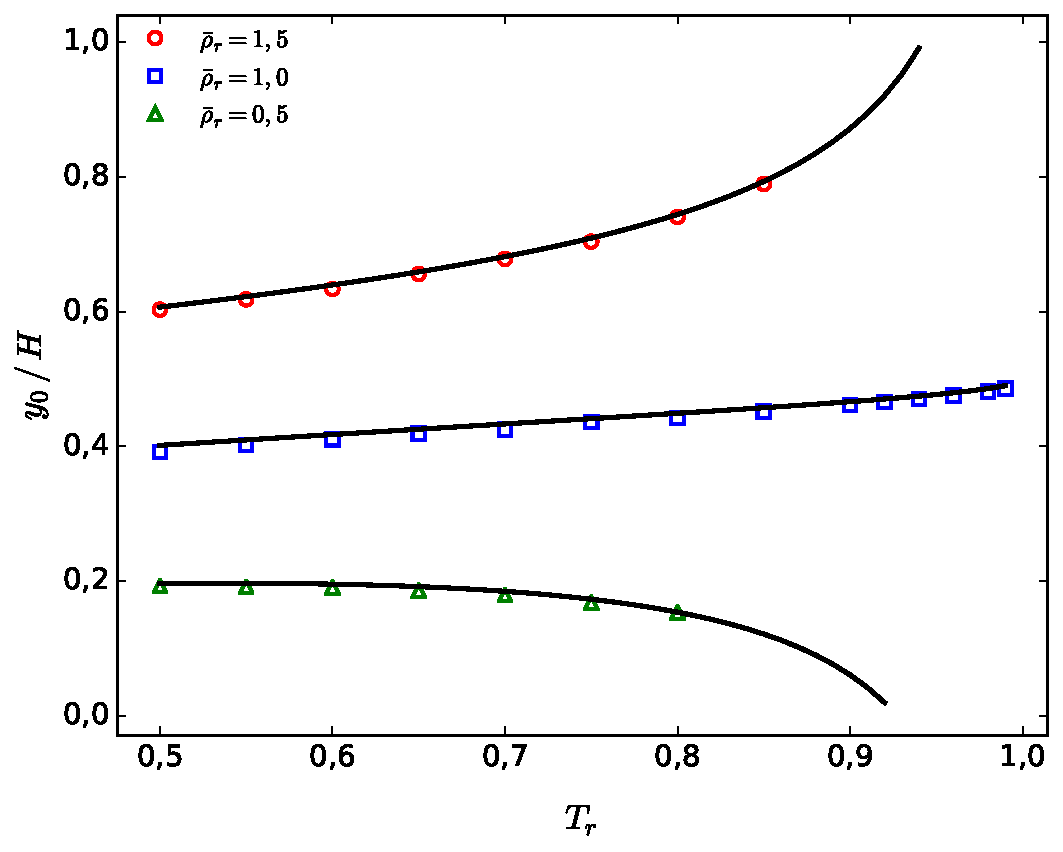
\includegraphics[width=0.75\textwidth]{vdWColumn/frac_volumen/frac_volumen}
	\caption{Posici\'on de la interfase  para diferentes temperaturas en una cavidad con $E_r(H)=10^{-3}$, empleando distintos valores de densidad inicial. Las l\'ineas continuas corresponden a la soluci\'on anal\'itica, mientras que los puntos representan  los resultados de la simulaci\'on con lattice Boltzmann.}
	\label{fig:vdWColumn_frac_volumen}
\end{figure}

Como se mencion\'o anteriormente, uno de los objetivos principales de la comparaci\'on con la soluci\'on anal\'itica consiste en cuantificar los efectos de la fuerza volum\'etrica en la inconsistencia termodin\'amica. Esta influencia puede analizarse a partir de la \fig{fig:vdWColumn_rhor_egrav}, donde se muestran los perfiles de densidad calculados para una cavidad con $T_r=0.99$ y diferentes valores de energ\'ia gravitacional m\'axima. En este caso, los cambios de $E_r(H)$ se reflejaron en las simulaciones a trav\'es de distintos valores de $g$, y los perfiles resultantes se muestran sobre una coordenada normalizada que refleja la distancia a la interfase, es decir, $(y-y_0)/H = (E_r-E_r(y_0)) / E_r(H)$. Como puede apreciarse en la \fig{fig:vdWColumn_rhor_egrav}, el uso de $\sigma=0.125$ permite obtener una representaci\'on adecuada de la distribuci\'on de densidad en el seno del fluido, incluso para valores de $E_r(H)$ elevados.

\begin{figure}[ht]
	\centering
	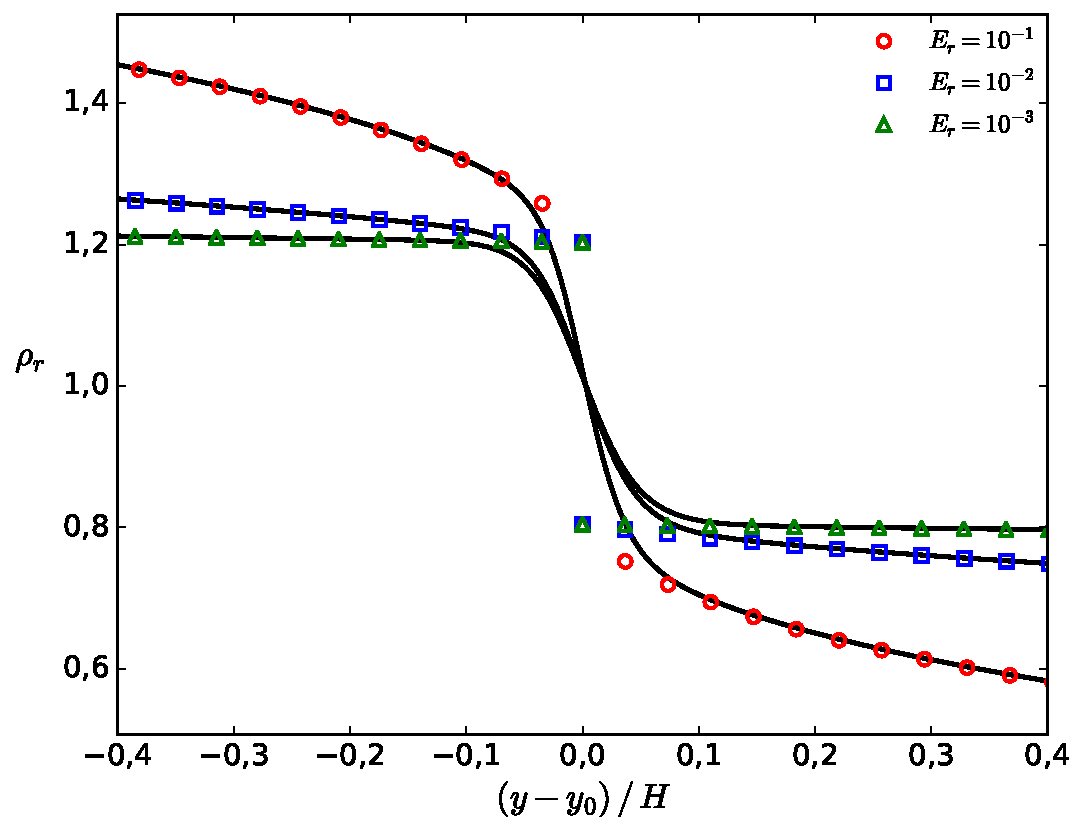
\includegraphics[width=0.75\textwidth]{vdWColumn/energia_grav/rhor_energia_grav}
	\caption{Perfiles de densidad para una cavidad con $T_r = 0.99$ y diferentes $E_r(H)$. Las l\'ineas s\'olidas corresponden a los resultados num\'ericos.}
	\label{fig:vdWColumn_rhor_egrav}
\end{figure}

En los perfiles de densidad mostrados en las \figs{fig:vdWColumn_rhor_tuniform}{fig:vdWColumn_rhor_egrav} se evidencia que, para la misma cantidad de unidades de grilla en la direcci\'on vertical ($H$) e iguales constantes de van der Waals, la resoluci\'on de la interfase recuperada empeora con el incremento de la temperatura. Por lo tanto, en este punto resulta v\'alido cuestionarse c\'omo es posible mejorar la precisi\'on de la simulaci\'on, que en este caso implica reducir el espesor de la interfase, ya que en el interior de cada fase la representaci\'on es adecuada para las grillas utilizadas.

La primera alternativa consiste en mantener la representaci\'on en unidades reducidas e incrementar $H$. De este modo, se mantienen sin cambios el resto de las contantes de la simulaci\'on a excepci\'on de $g$, que debe adaptarse para conservar el valor de energ\'ia gravitacional reducida m\'axima, $E_r(H) = 10^{-3}$. En la \fig{fig:vdWColumn_rhor_grilla} se observa que la representaci\'on del perfil de densidad reducida, sobre coordenadas adimensionales, produce una mejora consistente en la resoluci\'on de la interfase.

\begin{figure}[ht]
	\centering
	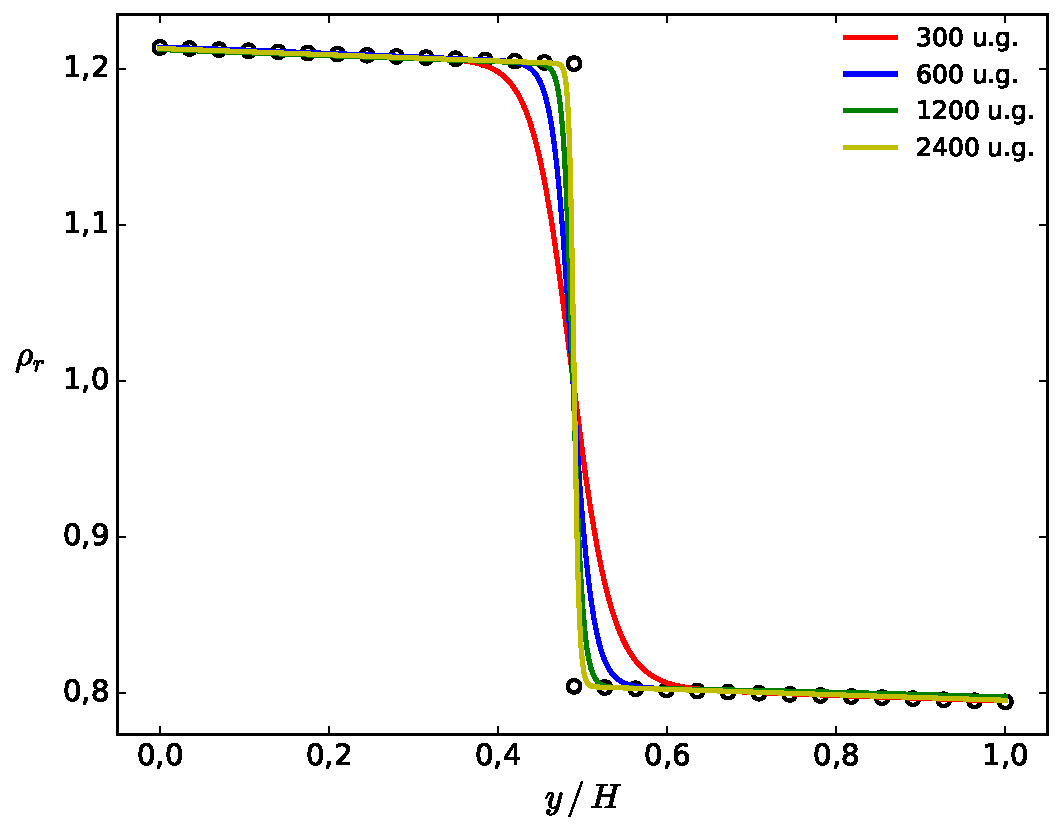
\includegraphics[width=0.75\textwidth]{vdWColumn/TUniform_grilla/rhor_Tuniform_grilla}
	\caption{Perfiles de densidad para una cavidad con $T_r = 0.99$, $E_r(H) = 10^{-3}$ y diferente cantidad de unidades de grilla en la direcci\'on vertical. Los puntos corresponden a la soluci\'on anal\'itica.}
	\label{fig:vdWColumn_rhor_grilla}
\end{figure}

Esta mejora significativa en la reproducci\'on de la interfase se debe, en parte, a que el espesor de la misma se mantiene constante en unidades de grilla, ya que depende exclusivamente de la temperatura reducida y las constantes de la ecuaci\'on de estado. Por lo tanto, es razonabe esperar que, para una misma $T_r$, $E_r(H)$ y $H$, el ancho de la interfase pueda reducirse usando diferentes valores para $a$ y $b$. Este efecto puede apreciarse en las \figs{fig:vdWColumn_b_eos}{fig:vdWColumn_a_eos}, donde se muestran los perfiles de densidad para una cavidad con $T_r=0.99$, $H=300$ y $E_r(H)=10^{-3}$, obtenidos con valores de $b$ fijos ($b=4$) y variando $a$, y viceversa ($a=0.5$). En ambos casos, ya sea incrementando $a$ o disminuyendo $b$, se produce una reducci\'on del espesor de la interfase en unidades de grilla mientras que se conservan los perfiles reducidos en el interior de cada fase. En particular, el incremento del par\'ametro $b$ produce un aumento en la diferencia de densidad absoluta entre cada fase. Por otro lado, el incremento de $a$ y la dismunuci\'on de $b$ contribuyen a incrementar el gradiente (dimensional) del potencial de interacci\'on. Ambos efectos contribuyen a mejorar la capacidad del modelo \pp{} para reproducir la interfase, y de esta forma producir una tendencia similar a la observada frente a un incremento en la resoluci\'on de grilla. Sin embargo, es necesario destacar que en este camino se observaron limitaciones de aplicabilidad relacionadas con la estabilidad de la simulaci\'on.

\begin{figure}[ht]
	\centering
	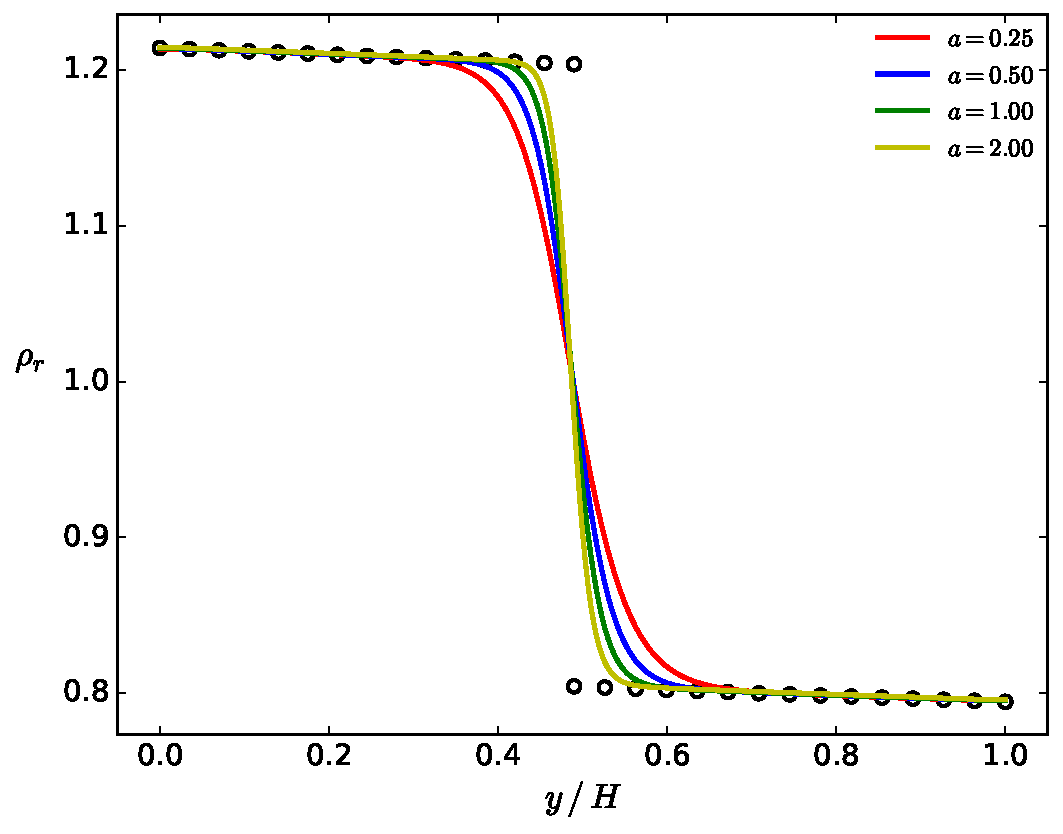
\includegraphics[width=0.75\textwidth]{vdWColumn/TUniform_a_eos/rhor_Tuniform_a_eos}
	\caption{Perfiles de densidad para una cavidad con $T_r = 0.99$, $E_r(H) = 10^{-3}$ y diferente cantidad de unidades de grilla en la direcci\'on vertical. Los puntos corresponden a la soluci\'on anal\'itica.}
	\label{fig:vdWColumn_b_eos}
\end{figure}

\begin{figure}[ht]
	\centering
	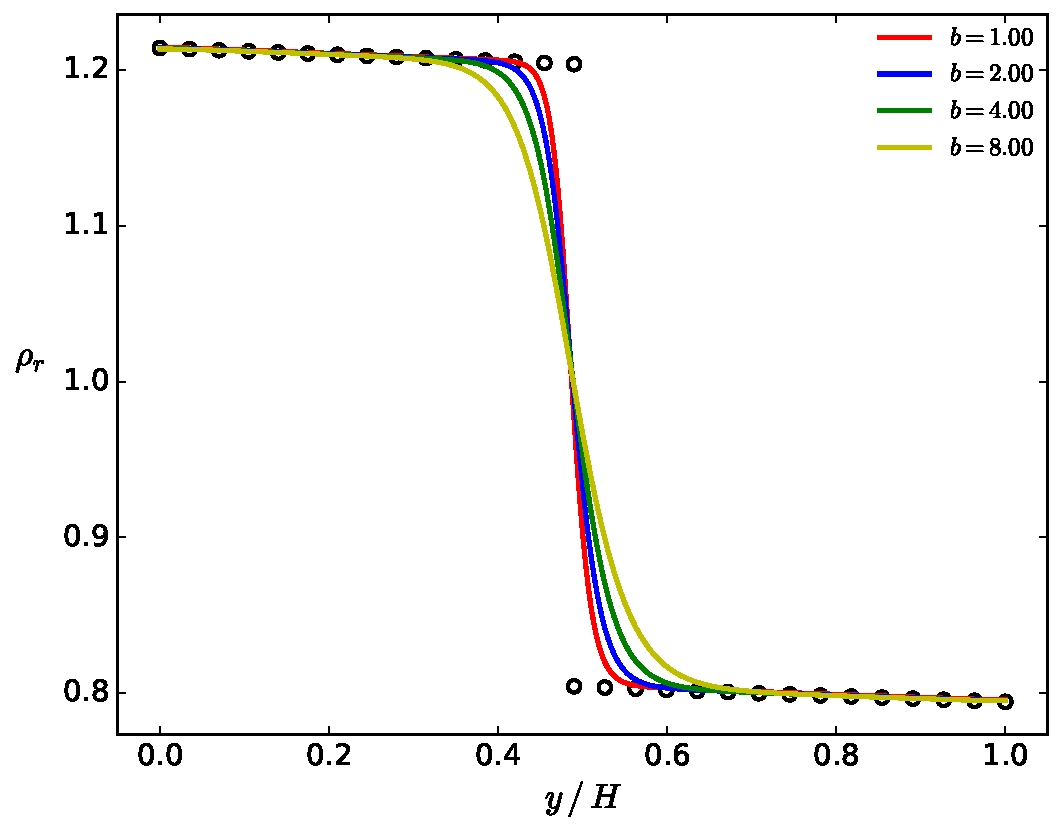
\includegraphics[width=0.75\textwidth]{vdWColumn/TUniform_b_eos/rhor_Tuniform_b_eos}
	\caption{Perfiles de densidad para una cavidad con $T_r = 0.99$, $E_r(H) = 10^{-3}$ y diferente cantidad de unidades de grilla en la direcci\'on vertical. Los puntos corresponden a la soluci\'on anal\'itica.}
	\label{fig:vdWColumn_a_eos}
\end{figure}
\FloatBarrier

La soluci\'on anal\'itica tambi\'en permite obtener perfiles de densidad en casos donde la distribuci\'on de temperatura no es uniforme. En una segunda prueba num\'erica se utiliz\'o $T_t=0.99$ y se consider\'o una distribuci\'on lineal de temperatura en la cavidad, variando param\'etricamente la temperatura de la cara inferior, $T_b$. El resto de las constantes y propiedades de simulaci\'on permanecen iguales a los casos anteriores.

En la \fig{fig:vdWColumn_rhor_TNonUniform} se muestran los perfiles de densidad obtenidos para diferentes $T_b$. Nuevamente, puede observarse que el modelo \pp{} es capaz de reproducir correctamente la distribuci\'on de densidad en el interior de cada fase, y genera una interfase cuyo espesor disminuye junto con la temperatura de la cara inferior.

\begin{figure}[ht]
	\centering
	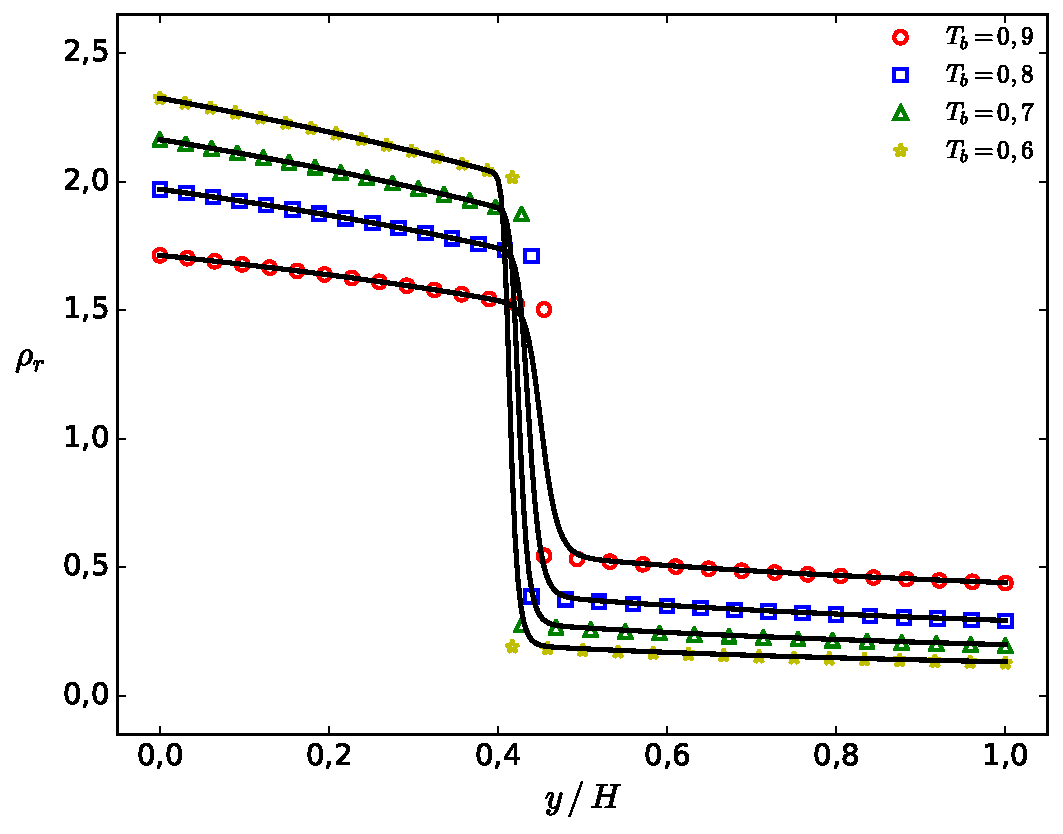
\includegraphics[width=0.75\textwidth]{vdWColumn/TNonUniform/rhor_vdWcolumn_TNonUniform}
	\caption{Perfiles de densidad para una cavidad con $T_t = 0.99$ y una distribuci\'on lineal de temperatura, fijada para diferentes valores de $T_b$. Los puntos corresponden a la soluci\'on anal\'itica.}
	\label{fig:vdWColumn_rhor_TNonUniform}
\end{figure}

Siguiendo la idea de la prueba num\'erica anterior, tambi\'en es posible verificar la consistencia de este m\'etodo \pp{} usando diferentes unidades de grilla en la direcci\'on vertical. Como puede apreciarse en la \fig{fig:vdWColumn_TNonUniform_grilla}, si se incrementa $H$ a la vez que se conservan los dem\'as par\'ametros adimensionales representativos, es posible lograr una reducci\'on consistente y precisa del espesor de la interfase sobre coordenadas adimensionales.

\begin{figure}[ht]
	\centering
	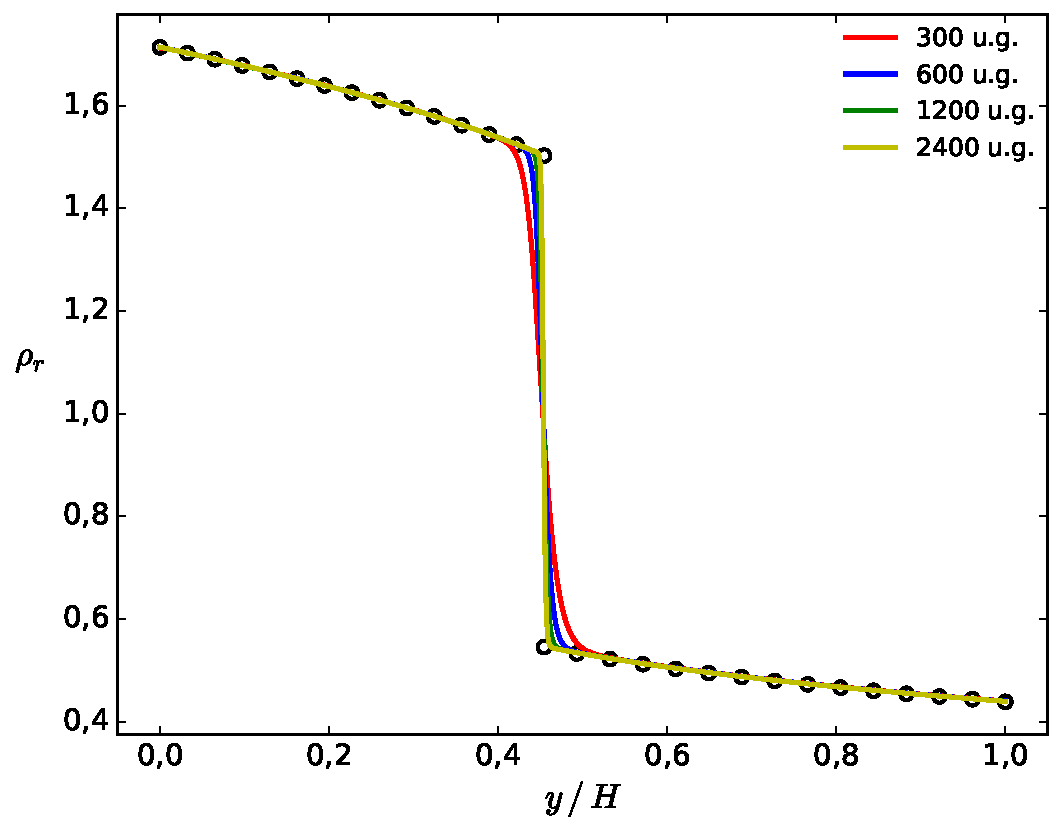
\includegraphics[width=0.75\textwidth]{vdWColumn/TNonUniform_grilla/rhor_TNonUniform_grilla}
	\caption{Perfiles de densidad para una cavidad con $T_t = 0.99$ y una distribuci\'on lineal de temperatura, con diferentes unidades de grilla en la direcci\'on vertical. Los puntos corresponden a la soluci\'on anal\'itica.}
	\label{fig:vdWColumn_TNonUniform_grilla}
\end{figure}


Los resultados num\'ericos muestran que el modelo \pp{} de Li et al. es capaz de reproducir el perfil de densidad dado por la soluci\'on anal\'itica, para diferentes condiciones de simulaci\'on. El par\'ametro $\sigma$ puede ajustarse libremente para compensar parcialmente el problema de la inconsistencia termodin\'amica, y as\'i obtener un acuerdo excelente en el seno de cada fase, junto con un perfil continuo de densidad en la zona d\'onde tiene lugar la segregaci\'on de fases. El espesor de esta interfase en unidades de grilla puede modificarse usando diferentes constantes en la ecuaci\'on de estado, o reducirse si se expresa adimensionalmente al incrementar la resoluci\'on de la grilla.

Estos efectos pueden analizarse como consecuencia de la ecuaci\'on de conservaci\'on de impulso lineal recuperada (\eq{eq:li_macro}), que en una situaci\'on unidimensional se reduce a:
\begin{equation}
	-\dfrac{\partial}{\partial y}(\rho c_s^2) + F_{i_y} + F_{b_y} - 2 G^2 c^4 \sigma \dfrac{\partial}{\partial y} \left( \left| \dfrac{\partial \psi}{\partial y} \right|^2  \right) = 0.
	\label{eq:li_macro_1d}
\end{equation}

La \fig{fig:vdWColumn_TUniform_fuerza} muestra los perfiles de la fuerza de interacci\'on y de $\psi d\psi / dy$, para una cavidad isot\'ermica con $T_r = 0.99$, $H=300$ y $E_r(H)=10^{-3}$. La fuerza graficada corresponde a la componente de la \eq{eq:f_int} en la direcci\'on $y$, mientras que el t\'ermino restante se calcul\'o usando la \eq{eq:potencial} y un esquema de diferencias centradas para las derivadas espaciales.

\red{completar}

\begin{figure}[ht]
	\centering
	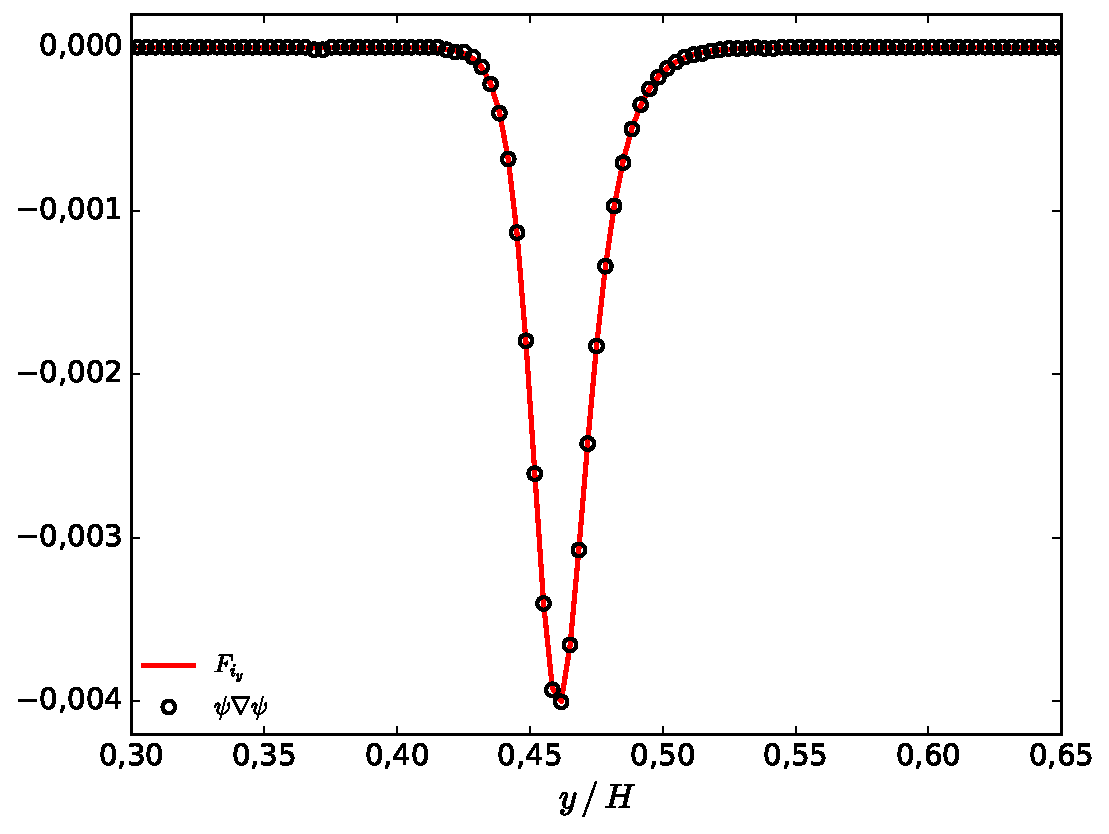
\includegraphics[width=0.75\textwidth]{vdWColumn/Fuerza/vdWcolumn_fuerza}
	\caption{Perfiles de densidad para la fuerza de interacci\'on y $\psi d\psi / dy$.}
	\label{fig:vdWColumn_TUniform_fuerza}
\end{figure}

En este caso, es necesario notar que de acuerdo a la \eq{eq:f_int_taylor}, el t\'ermino de fuerza de interacci\'on satisface $F_{i_y} = -Gc^2 \psi d\psi / dy$, y por lo tanto la \eq{eq:li_macro_1d} puede escribirse como:
\begin{equation}
	-\dfrac{\partial p_{EOS}}{\partial y} + F_{b_y} - 2 G^2 c^4 \sigma \dfrac{\partial}{\partial y} \left( \left| \dfrac{\partial \psi}{\partial y} \right|^2  \right) = 0.
	\label{eq:li_macro_1d_peos}
\end{equation}

La \eq{eq:li_macro_1d_peos} es similar al balance hidrost\'atico empleado por Berberan-Santos (\eq{eq:p_hidrost}) excepto por el t\'ermino adicional $- 2 G^2 c^4 \sigma \frac{\partial}{\partial y} \left( \left| \frac{\partial \psi}{\partial y} \right|^2  \right)$. La \fig{fig:vdWColumn_fuerza_terminos} muestra la importancia de los diferentes t\'erminos de la \eq{eq:li_macro_1d}. A pesar que esta ecuaci\'on es igual a la \eq{eq:f_int_taylor} an casi todo el dominio, $- 2 G^2 c^4 \sigma \frac{\partial}{\partial y} \left( \left| \frac{\partial \psi}{\partial y} \right|^2  \right)$ es diferente de cero s\'olo en las cercan\'ias de la interfase, y aunque es de un orden de magnitud menor que los principales t\'erminos de la \eq{eq:li_macro_1d}, es capaz de afectar el comportamiento de las variables macrosc\'opicas para producir el perfil de densidad continuo y difuso a trav\'es de la interfase.


\begin{figure}[ht]
	\centering
	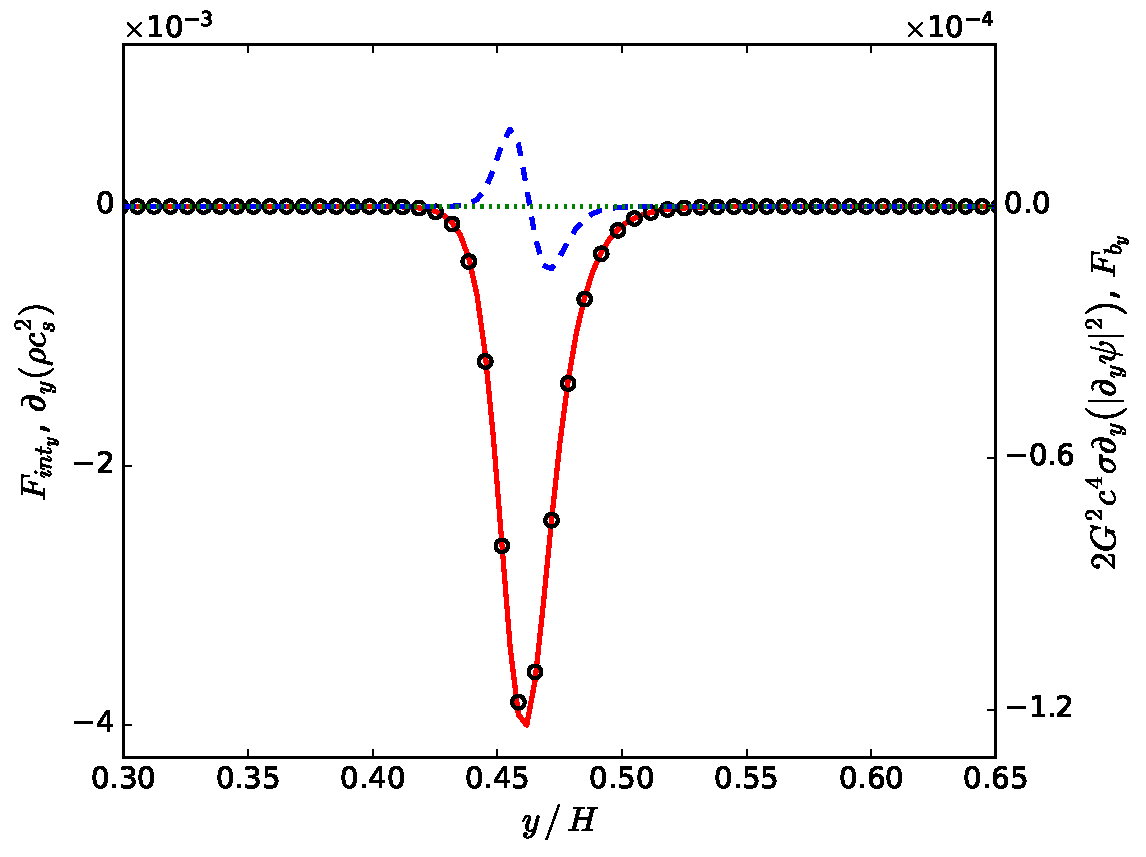
\includegraphics[width=0.75\textwidth]{vdWColumn/Fuerza_componentes/vdWcolumn_fuerza_comp}
	\caption{\red{Hay que corregir la figura. Ubicar leyenda manualmente y noteci\'on cient\'ifica}}
	\label{fig:vdWColumn_fuerza_terminos}
\end{figure}


\red{Resumen y conclusiones. Resumir ideas obtenidas de este benchmark.}